\documentclass[UTF8,zihao=-4,a4paper,fontset=windows]{ctexart}
% 内置ctex基线初始化后按本地华为杯论文格式调整。
\usepackage{amsmath,amssymb,booktabs,array,longtable,tabularx}
\usepackage{geometry,graphicx,float,caption,tikz}
\usepackage{xcolor,listings,seqsplit,multicol}
\usetikzlibrary{arrows.meta,positioning,fit,calc}
\usepackage[hidelinks]{hyperref}
\geometry{left=2.5cm,right=2.5cm,top=2.5cm,bottom=2.5cm}
\ctexset{section={format=\centering\heiti\zihao{4}},subsection={format=\heiti\zihao{-4}},subsubsection={format=\heiti\zihao{-4}}}
\pagestyle{plain}
\linespread{1}
\setlength{\parindent}{2em}
\setlength{\emergencystretch}{2em}
\setlength{\textfloatsep}{14pt}
\setcounter{tocdepth}{3}
\captionsetup{font=normalsize,labelsep=quad}
\renewcommand{\arraystretch}{1.2}
\newcolumntype{Y}{>{\raggedright\arraybackslash}X}
\newcommand{\keywords}[1]{\par\noindent\textbf{关键词：}#1}
\renewenvironment{abstract}{\begin{center}\heiti 摘\quad 要\end{center}}{\par}
\newcommand{\lexmin}{\mathop{\mathrm{lexmin}}}
\newcommand{\ind}{\mathbf{1}}
\tikzset{block/.style={draw=blue!50!black,fill=blue!5,rounded corners=2pt,align=center,text width=3.1cm,minimum height=1cm,font=\small},edge/.style={-{Stealth[length=2mm]},thick,draw=blue!55!black}}
\lstdefinestyle{pythonappendix}{
  language=Python,
  basicstyle=\ttfamily\scriptsize,
  keywordstyle=\color{blue!60!black},
  commentstyle=\color{green!40!black},
  stringstyle=\color{orange!55!black},
  numbers=left,
  numberstyle=\tiny\color{gray},
  numbersep=7pt,
  frame=single,
  rulecolor=\color{gray!45},
  breaklines=true,
  breakatwhitespace=false,
  columns=fullflexible,
  keepspaces=true,
  showstringspaces=false,
  tabsize=4,
  xleftmargin=1.5em,
  framexleftmargin=1.2em,
  aboveskip=8pt,
  belowskip=10pt
}
\begin{document}
\begin{center}
{\heiti\zihao{3}山区应急物资运输与通信保障的协同建模}\par\medskip
吃炸家
\end{center}
\begin{abstract}
山区洪涝灾害会同时破坏道路通行条件和地面通信覆盖，使应急物资投送从单纯的最短路问题转化为地形、能量、时限、装备周转和连续通信共同约束的协同决策问题。题目给出15个服务区、80个不可拆货箱、三类运输无人机及共享电池，并允许在直连通信不足时使用中继无人机。本文按照“单点能力标定—多点运输调度—运输通信协同—独立任务分区”的递进关系，建立统一的航段、能耗和资源事件模型。模型始终以硬约束可行为第一层目标，再比较一般物资及时性、任务完成时间、能耗和架次数。

针对问题一，首先沿每条航段遍历实际经过的30~m DEM像元，以最高地形加50~m确定巡航海拔；结合载荷相关等效航程、爬升能耗和返航安全余量，利用二分法求解“服务区—机型”最大安全载荷。随后枚举满足质量、体积和能量约束的完整货箱子集，以架次数、能耗和累计作业时间为字典序代价，通过集合划分动态规划获得单点组批方案。结果表明，45个“服务区—机型”组合均可空载返航，但B型和C型在部分远距或高地形节点受到能量限制；全体物资共需18架次，累计能耗59.240~kWh，累计作业时间9.111~h。18个批次中，体积、质量和能量分别成为9、5和4个批次的最紧约束，说明不可拆货箱条件下仅按额定载质量估计架次数会产生偏差。

针对问题二，将货箱组批、访问顺序、机型、实体机、共享电池和开始时刻置于同一事件时间轴。逐站递推交付时刻与剩余载荷，医疗及首批保障货箱采用硬截止约束，一般物资采用归一化加权迟到指标；实体机占用至返航，电池则占用至两阶段充电结束。求解时分别构造硬箱专送基线与同目的地混装方案，通过软箱补入、单区精确组批和双区串访形成两套候选，并由事件仿真器完成资源排程。与26架次硬箱专送基线相比，所选混装方案以22架次完成80箱唯一交付，31个硬时限箱均无违约，一般物资超期箱由23箱降至9箱，$WTD$由111.492降至38.787；完成时间为2.679~h，总能耗为69.602~kWh，分别较基线下降24.1\%和16.2\%。

针对问题三，依据双向链路预算、自由空间损耗和DEM视线遮挡建立直连与单中继可用判据，将运输轨迹展开为爬升、巡航、下降和交接区间。中继悬停点须同时满足边界、回传链路、往返能量和300~m离地高度要求；中继任务计入准备、飞抵、建链、悬停通信、返航、周转和能源组件充电。本文以问题二路线为已验证候选，采用离线筛选后固化的六个点位和七个波次组织中继资源，并用连续区间证书进行全时段认证，0.5~s网格仅作为独立复核。最终22个运输架次被组织为7个波次，配置11个中继架次，由2架中继机和5套能源组件执行；68个通信分段包含41段直连和27段中继，连续认证无未解析区间，65532个加密采样点无中断。联合完成时间为6.572~h，总能耗79.097~kWh，最小保守链路余量为0.1397~dB。该结果证明当前方案可行，但不构成运输—通信全局最优性证明。

针对问题四，冻结问题三的组批、路线、时序和实际通信指派，以同架次共访关系构造服务区图，得到11个不可拆原子块；对每个合法分区，从通信分段反推组内中继任务，并以固定占用区间的峰值并发数计算各类资源最小配置。实际穷举1023个两组候选和57002个三组带标签候选，后者对应28501个无标签等价类。结果表明：两组最优方案不产生库存缺口，三组最优方案需要额外增加1架中继无人机，并相对集中执行多配置1套中继能源组件。因此，在“先消除库存缺口，再减少总配置并改善均衡”的评价准则下选择两组方案；若强调区域自治，则需接受额外资源。

模型从航段像元、逐架次能量、80箱唯一覆盖、资源无冲突和连续通信五个层次进行检验。敏感性实验表明：返航余量提高至25\%会使问题一架次数由18增至19；既定问题二方案在1200~s事件延误内仍满足硬时限；问题三原证书可承受0.1~dB附加损耗。本文以统一事件时间轴贯通运输、能源和通信，使结论能够回溯到具体货箱、架次或时间区间。

\keywords{应急物资运输；集合划分动态规划；共享电池调度；连续通信认证；任务分区}
\end{abstract}

\clearpage
\begin{center}{\heiti\zihao{4}目\quad 录}\end{center}
\vspace{-0.8em}
\begingroup
\scriptsize
\renewcommand{\baselinestretch}{0.90}\selectfont
\setlength{\parskip}{0pt}
\begin{multicols}{2}
\raggedcolumns
\makeatletter\@starttoc{toc}\makeatother
\end{multicols}
\endgroup
\clearpage
\section{问题重述与总体分析}
\subsection{场景与研究任务}
本文以赛题给定的镇龙乡及周边山区标准场景为研究对象\textsuperscript{\cite{D2026}}。调度中心O01负责向15个服务区配送80个不可拆货箱，物资包括饮用水、应急食品、医疗物资和生活卫生用品。可用运输装备由三种机型、八架实体无人机和配套共享电池组成；在固定网关不能提供直接通信的区域，还可调用中继无人机与可更换能源组件。

运输方案的可执行性由空间、时间和资源共同决定。空间上，航段须保持沿线地形净空，山地爬升会改变能耗；时间上，医疗箱和首批保障箱受硬截止约束，其他货箱存在及时性要求；资源上，同一架无人机不能同时执行多个任务，电池返航后也不能立即视为满电。通信进一步把运输轨迹和中继在位时段联系起来：一条路线即使能量可行，也可能因某段飞行缺少可用链路而不可执行。

\subsection{四个问题的层次与衔接}
问题一在单服务区直接往返条件下研究运输能力和组批。每个服务区单独处理，既不跨服务区拼箱，也不安排具体实体机和电池。其作用是建立一致的航段计算规则，得到单点任务的容量边界和可行批次。

问题二允许同一架次访问多个服务区，联合确定组批、访问顺序、机型、实体机、电池与开始时刻。多点串访可减少重复往返，但增加后续货箱的等待，并改变各航段的剩余载荷。因此，不能只比较总里程，也不能把问题一的架次直接并行排列后视为调度完成。

问题三把连续通信加入问题二。中继任务需提前飞抵并完成建链，服务结束后还要返航，其在位时长同时受到能源和设备周转限制。运输开始时刻变化会移动通信需求区间；中继不可及时就位时，则需要调整运输时序或任务组织。

问题四以有效的问题三联合方案为固定输入，分别划分两个和三个独立任务组。此时研究重点从重新优化路线转向固定任务的归属与资源核算。同架次共访的服务区必须同组，跨组资源不得调配，通信保障关系也不能随分组任意改写。

上述依赖关系见图\ref{fig:overall}。四问共用节点编号、物理参数、能耗与时间口径；后一问增加约束或改变执行组织形式，但不另设一套基础计算规则。
\begin{figure}[H]\centering
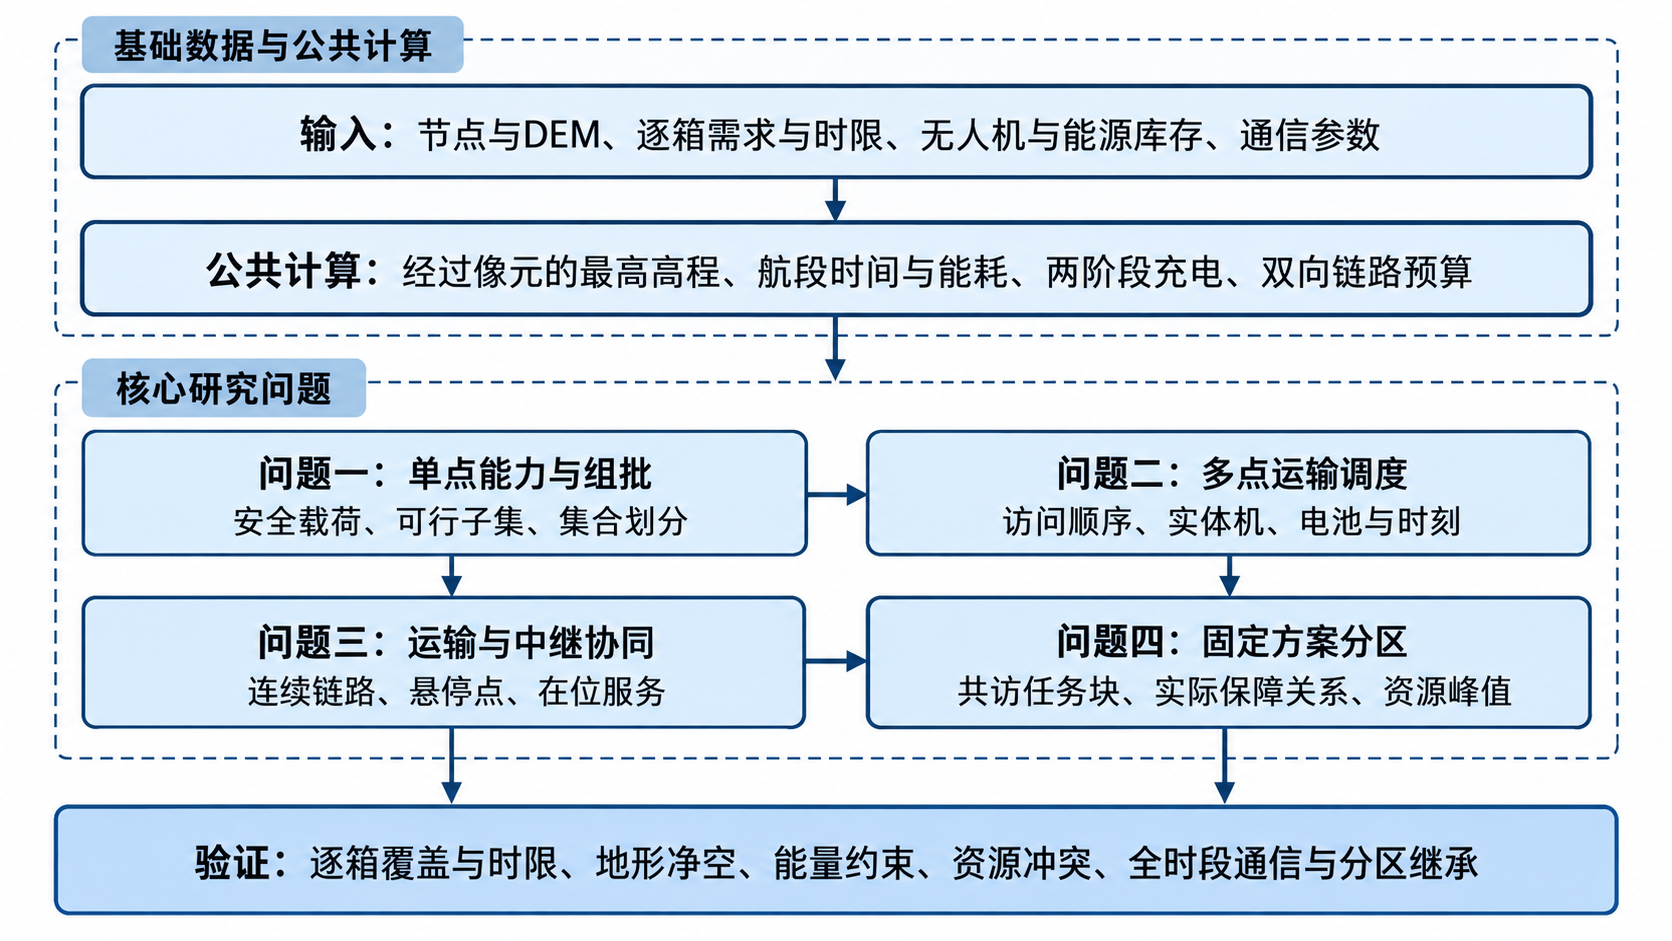
\includegraphics[width=.86\textwidth]{figures/common/figure1.png}
\caption{四个子问题的输入、方法与输出依赖关系}\label{fig:overall}
\end{figure}

\subsection{研究策略与评价原则}
本文采用可行性优先的建模策略。载质量、装载体积、返航电量、硬截止以及资源占用构成不可违反的约束；在可行集合内，再比较迟到、完工时间、能耗和架次数。这样可以避免通过降低安全余量或容忍医疗箱逾期，换取表面上的目标改善。

不同层次的最优性应分别表述。单点组批可在完整候选集合上进行精确动态规划；多点运输与中继联合调度采用构造与事件仿真方法时，只能说明所获候选方案的表现。固定时序下的任务分区若穷尽全部合法划分，可讨论该固定方案及所选评价口径下的最优分区，不能据此推及整体运输通信问题的全局最优。

\section{模型假设与符号说明}
\subsection{模型假设及适用条件}
\begin{enumerate}
\item 需求、时限、机型性能及能源库存以附件为准，采用确定性离线计划。模型不描述任务开始后的新增需求、设备故障或临时空域封闭；这些因素应在后续情景分析中单独引入。
\item 航段按照题面规定的水平直线执行，服务区投送后重新从作业高度爬升。道路、水系等地理数据用于解释空间背景，不以道路长度代替空中航段距离。
\item 给定等效航程对应单组可用能量的标准水平航程，水平能耗按距离占等效航程的比例折算；爬升附加能耗按重力势能与效率计算。此为对题面能耗分项的建模解释，保持量纲闭合，不另加未给定的下降能量回收。
\item 未获得气象时序时，飞行速度与能耗按名义参数计算。无风修正不是对山区实际气象的判断，而是当前输入条件下的计算边界。
\item 每个中继架次采用一个静态悬停点，服务前完成建链。题面未给出并发接入容量上限，因此允许同一在服中继保障多个运输架次，但每一条接入链路和回传链路仍需同时满足可用条件。
\item 问题四保持问题三的绝对任务时序、访问顺序和实际通信指派。若一个中继任务确实服务多个任务组，则在相关组中分别配置能够执行该完整任务的资源，不截取局部服务片段来降低主方案需求。
\end{enumerate}
地形净空、能量余量、医疗与首批时限属于题目约束，不能通过假设放宽；对风场、突发需求等缺失信息，应在适用边界中说明，而不能补造参数。

\subsection{主要符号}
表\ref{tab:symbols}列出主要符号。实体无人机、机型、架次和航段分别表示不同层次的对象；时间采用相对任务起点的秒数，能量采用kWh。
\begin{longtable}{p{2.8cm}p{8.5cm}p{1.8cm}}
\caption{主要符号、含义与单位}\label{tab:symbols}\\
\toprule 符号 & 含义 & 单位\\\midrule\endfirsthead
\toprule 符号 & 含义 & 单位\\\midrule\endhead
$S_i$ & 第$i$个服务区，$i=1,\ldots,15$ & —\\
$b,r,h$ & 货箱、运输架次、中继架次索引 & —\\
$g,u,k$ & 运输机型、实体运输机、共享电池索引 & —\\
$w_b,v_b$ & 单箱质量与体积 & kg，m$^3$\\
$Q_g,V_g$ & 最大载货质量与装载体积 & kg，m$^3$\\
$m_g^0,q_{ij}$ & 含电池空载质量、航段剩余有效载荷 & kg\\
$d_{ij}$ & 节点间水平直线距离 & m\\
$H_i^{op},H_{ij}^{c}$ & 作业海拔、计划巡航海拔 & m\\
$h_{ij}^{+},h_{ij}^{-}$ & 爬升高度、下降高度 & m\\
$L_g(q)$ & 当前载荷下的等效航程 & m\\
$E_g^{use},E_r$ & 电池可用能量、运输架次能耗 & kWh\\
$\rho_g$ & 返航安全能量余量比例 & 1\\
$s_r,C_b$ & 架次准备开始时刻、逐箱交付完成时刻 & s\\
$d_b^{hard},d_b^{exp}$ & 有效硬截止、期望交付时刻 & s\\
$\alpha_b$ & 应急优先系数 & 1\\
$C_{max}$ & 所有相关任务最后返航时刻 & s\\
$T^{full}$ & 能源资源等效完全充电时间 & s\\
$\beta_{abt}$ & 端点$a,b$在时刻$t$的地形遮挡变量 & 0/1\\
$L_{ab}^{max}$ & 两通信方向中较小的允许传播损耗 & dB\\
$M^{link}$ & 链路预算与实际传播损耗之差 & dB\\
$H_p^R,h_p^{AGL}$ & 中继悬停海拔、悬停离地高度 & m\\
$n_{ka},I_a$ & 组$k$对资源$a$的需求、全局库存 & 架或组\\
$D_a^{(K)},R_a^{(K)}$ & $K$组分区的资源缺口、相对集中执行的冗余 & 架或组\\
$CV_W$ & 组间资源占用工作量的变异系数 & 1\\
\bottomrule\end{longtable}

\section{数据特征与公共物理模型}
\subsection{数据来源与统一口径}
\paragraph{（1）数据对象及其关联关系}
节点、货箱、运输机、中继机和通信参数分别由五份工作簿提供，地形由30米DEM描述\textsuperscript{\cite{Data2026}}。表\ref{tab:inputs}给出参与建模的对象规模。逐箱货箱清单作为分配的最小粒度，需求汇总表用于交叉核对；不能同时把两张表中的需求累加。
\begin{table}[htbp]\centering
\caption{标准场景的数据与资源构成}\label{tab:inputs}
\begin{tabularx}{\linewidth}{lYl}\toprule
对象 & 计算用途 & 规模\\\midrule
调度节点 & 航段、投送与网关定位 & 1个中心、15个服务区\\
逐箱需求 & 不可拆分配送与逐箱时限 & 80箱、53条汇总记录\\
运输无人机 & 机型选择与实体调度 & A/B/C共8架\\
运输电池 & 同型共享与充电周转 & A/B/C共14组\\
中继设备 & 空中接入与网关回传 & 2架、6组能源组件\\
DEM & 最高地形与视线遮挡 & $1309\times1486$像元\\
\bottomrule\end{tabularx}\end{table}

节点与需求空间关系见图\ref{fig:service-map}。点位决定飞行距离，点面积反映需求质量；二者共同影响组批，但尚不能据此判断某节点需要多少架次，因为安全载荷还受爬升和返航余量约束。
\begin{figure}[htbp]\centering
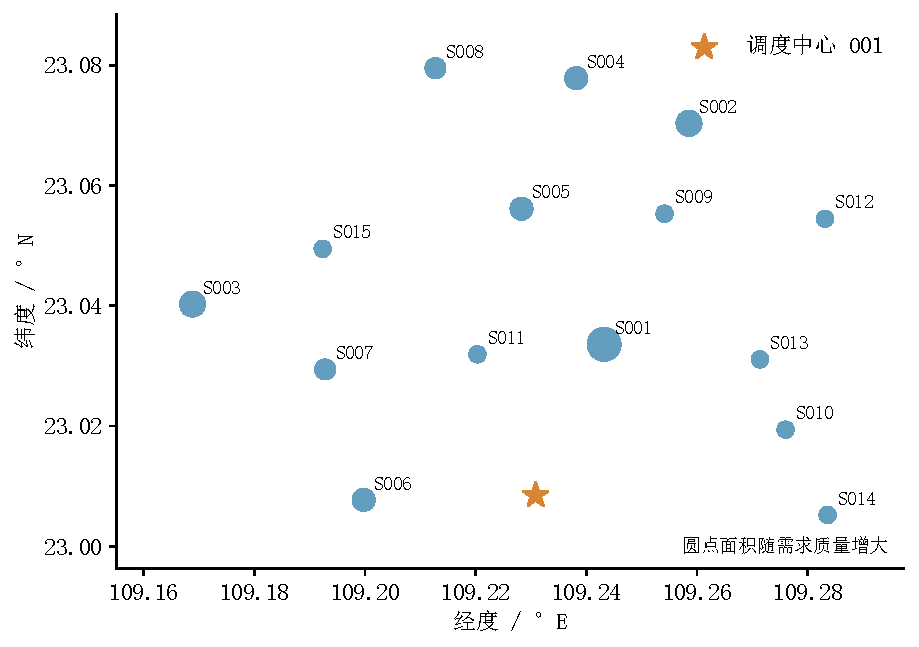
\includegraphics[width=.86\linewidth]{figures/data/raw_service_map.pdf}
\caption{调度中心与服务区分布：依据附件节点坐标与逐区需求绘制}
\label{fig:service-map}\end{figure}

\subsection{数据预处理与质量控制}
\paragraph{（1）编号、单位与缺失值处理}
不同附件以节点、货箱、机型和实体设备作为主键。预处理首先统一去除编号两端空格，保留前导零，并检查服务区编号是否属于S001--S015、中心与网关是否对应O01和G01。货箱目的地必须能在节点表中找到，实体无人机与电池必须能映射到A/B/C机型，中继能源组件则单独编号。任何无法建立外键关系的记录都不进入求解，而应回到原始附件核查。

质量统一为kg、体积统一为m$^3$、距离统一为m、时间内部统一为s、能量统一为kWh、功率统一为kW。经纬度仅用于空间定位，进入距离和DEM索引前转换为弧度或像元坐标；通信计算再把三维距离换算为km，以匹配自由空间损耗公式中的常数。单位转换在数据入口完成，避免在各子问题中重复换算产生口径漂移。

对关键字段执行非空和范围检查：货箱质量体积必须为正；机型容量、可用能量、速度和效率必须在物理允许范围内；SOC和安全余量位于$[0,1]$；中继离地高度不超过300~m。题目附件中的确定参数不采用均值填补。若关键值缺失，相关对象被标记为不可计算，而不是由相邻记录推测。

\paragraph{（2）需求汇总与双向核对}
逐箱清单是优化模型的权威需求源，因为不可拆货箱、类别、优先系数和时限均定义在箱级。需求汇总表只用于检查：按服务区聚合逐箱质量、体积和箱数后，应与汇总记录一致；再按物资类别核对医疗箱、首批保障箱及其交集。式\eqref{eq:hard-count}中的31箱来自集合并集，而不是简单相加。

求解输出也执行反向核对。问题一和问题二完成后，将结果表按货箱编号展开，要求原始80个编号与输出80个编号集合完全相同，且每个编号出现次数恰为1；按服务区重新汇总质量和体积，应回到输入值。该双向检查能够发现“总箱数正确但某箱重复、另一箱遗漏”的隐蔽错误。

\paragraph{（3）空间数据与DEM配准}
DEM栅格通过其经纬度范围和行列数建立地理坐标到像元索引的映射。由于栅格行方向通常与纬度增加方向相反，预处理需分别验证四角坐标和中心点索引，避免把南北方向翻转。节点若落在DEM范围外应立即报错；航段若穿越边界，则该路线不能直接按现有DEM证明净空。

固定步长采样可能跳过恰好位于两采样点之间的高程像元。本文除15~m密集采样外，计算航线与经纬向半像元边界的交点，再在相邻交点间取中点，从而枚举直线实际穿过的最近邻像元。对每一航段保存最高像元高程及其索引，既用于巡航海拔，也用于后续通信视线检查。

表\ref{tab:data-quality}汇总从编号关联、需求守恒到DEM配准和输出覆盖的主要质量控制规则，并说明各类异常会影响哪一层模型。
\begin{table}[htbp]\centering
\caption{数据质量控制规则及其对模型的影响}\label{tab:data-quality}
\small
\begin{tabularx}{\textwidth}{>{\raggedright\arraybackslash}p{2.7cm}YY}
\toprule
检查对象 & 质量控制规则 & 未通过时的影响\\
\midrule
节点与货箱编号 & 主键唯一；货箱目的地必须存在于节点表 & 无法完成任务归属，停止求解并核对附件\\
需求守恒 & 逐箱汇总与服务区汇总的箱数、质量、体积一致 & 不能用汇总表替代逐箱表，也不能重复累计\\
机型与实体资源 & 每架实体机和电池映射到唯一机型，数量与库存表一致 & 会造成错误的容量或并发资源上限\\
时间与单位 & 秒、小时、kg、m$^3$、kWh、kW在入口统一 & 会直接改变能耗、充电或截止判断\\
DEM范围与方向 & 节点在栅格内；四角与中心索引方向核对 & 会造成航段最高地形和视线遮挡错误\\
输出覆盖 & 80箱各出现一次，目的地和原始记录一致 & 发现遗漏、重复或错误交付即判方案无效\\
\bottomrule
\end{tabularx}\end{table}

\subsection{需求结构与时限分类}
\paragraph{（1）硬时限集合的构造}
逐箱统计得到总质量758 kg、总体积2.011 m$^3$。其中医疗箱16箱，首批保障箱30箱，二者交集15箱，故具有至少一种硬时限要求的货箱数为
\begin{equation}N_{hard}=16+30-15=31.\label{eq:hard-count}\end{equation}
余下49箱使用期望送达时间计算软迟到。交集不能重复计数：同一货箱既为医疗物资又为首批保障时，应取两个适用截止时刻的较小值，而不是将其视为两项配送任务。

\paragraph{（2）需求规模与紧迫性分布}
图\ref{fig:demand}同时展示需求质量和硬软时限构成。这一组合图把载荷规模与时间紧迫程度并列，便于识别“质量较大”与“必须尽早送达”并非同一概念。图\ref{fig:deadlines}进一步区分仅医疗、仅首批、两者兼有和一般物资；相同坐标的样本合并表示，避免重叠掩盖数量。

从逐区统计可见，S001拥有15箱、154 kg需求，约占总质量的20.3\%；S009至S015各有3箱、25 kg需求。S001的硬时限箱为3箱，其余服务区均为2箱，说明需求质量的差异明显大于硬时限箱数量的差异。调度时需要既给各区配置早期保障，又为大需求节点安排后续运力，不能仅按总质量大小排序服务。
\begin{figure}[htbp]\centering
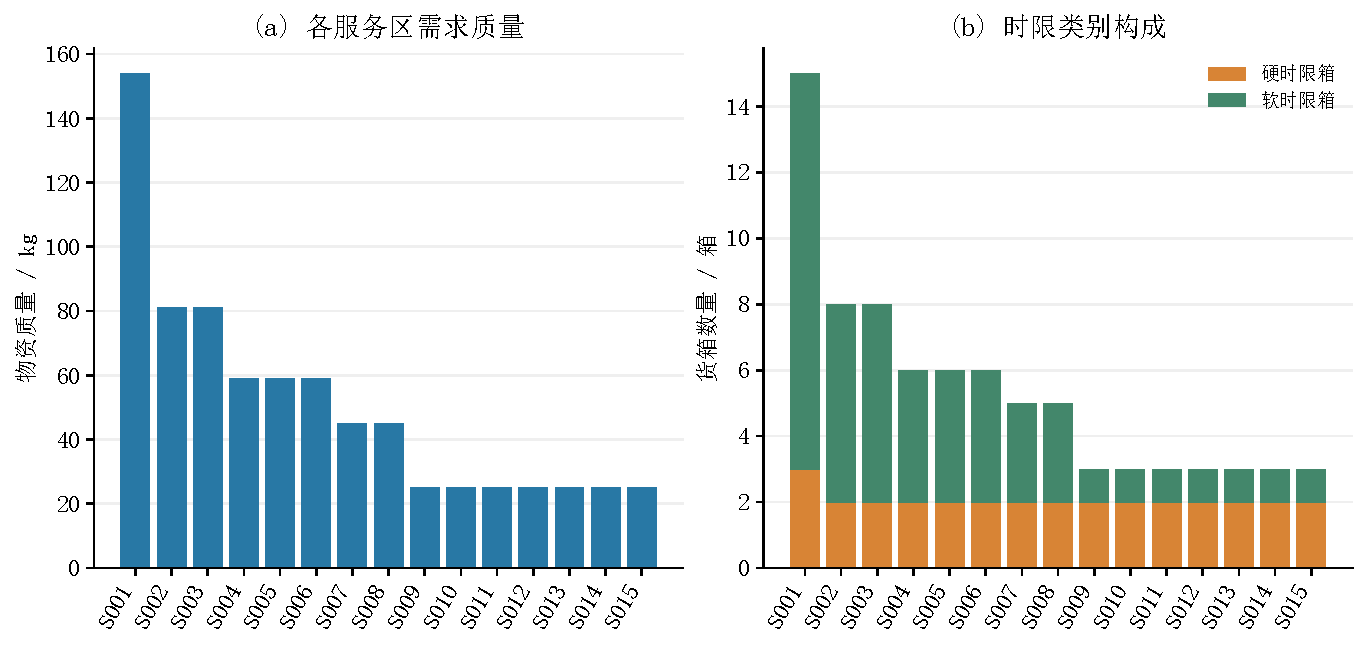
\includegraphics[width=\linewidth]{figures/data/raw_demand_composition.pdf}
\caption{各服务区的需求质量及硬软时限货箱构成}\label{fig:demand}\end{figure}
\begin{figure}[htbp]\centering
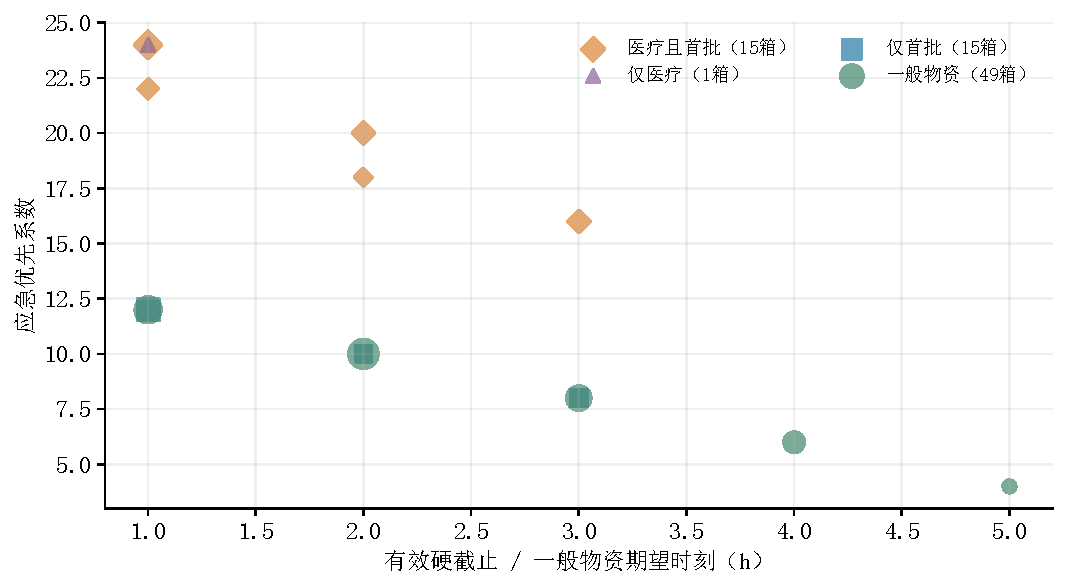
\includegraphics[width=.9\linewidth]{figures/data/raw_deadline_classes.pdf}
\caption{时限与优先系数：硬时限箱采用有效截止，一般物资采用期望时刻；点面积随同坐标箱数增大}\label{fig:deadlines}\end{figure}

\subsection{异构机型与能源库存}
\paragraph{（1）容量差异与资源数量}
三类机型的容量和库存见表\ref{tab:types}。C型具有较大的额定载质量和体积，但不能仅凭容量判定其在所有节点最优：不同载荷下的等效航程、爬升质量和实体数量均会影响调度。共享电池总数包含初始装机与备用电池，不能再额外加上实体机数量。
\begin{table}[htbp]\centering
\caption{运输机型容量与同型资源库存}\label{tab:types}
\begin{tabular}{lrrrrr}\toprule
机型 & 载质量/kg & 体积/m$^3$ & 能量/kWh & 实体机/架 & 电池/组\\\midrule
A & 25 & 0.060 & 4.5 & 4 & 6\\
B & 30 & 0.073 & 4.0 & 2 & 4\\
C & 80 & 0.250 & 8.0 & 2 & 4\\\bottomrule
\end{tabular}\end{table}

\paragraph{（2）数据特征对模型设计的影响}
需求和装备数据共同决定四问的建模结构。80箱不可拆要求保留箱级决策；15个服务区、且单区最多15箱，使问题一可以按目的地分解并精确枚举；8架实体运输机和14块电池使问题二必须区分机体返航与电池充满；两架中继机和六套能源组件则限制问题三波次的并发数量。表\ref{tab:feature-model}概括从数据特征到模型模块的对应关系。

\begin{table}[htbp]\centering
\caption{关键数据特征与模型模块的对应关系}\label{tab:feature-model}
\begin{tabularx}{\textwidth}{YY Y}
\toprule
数据或题设特征 & 直接影响 & 对应模型处理\\
\midrule
货箱不可拆、箱级时限 & 不能用连续流量替代具体货箱 & 子集枚举、唯一覆盖和逐箱交付时刻\\
机型容量与载荷航程不同 & 有效载荷随节点和地形变化 & 安全载荷二分与逐段剩余载荷能耗\\
实体机少于任务数 & 多架次必须在时间轴上复用 & 实体机占用区间与事件排程\\
电池可跨同型机共享 & 机体可用不等于原电池可用 & 电池独立编号、SOC和两阶段充电\\
直连存在地形遮挡 & 距离近不一定链路可用 & DEM视线、双向预算和连续区间认证\\
任务组间资源不共享 & 分区会重复配置峰值资源 & 原子块分区和分组独立区间峰值\\
\bottomrule
\end{tabularx}\end{table}

\subsection{航段、地形净空与飞行时间}
\paragraph{（1）水平距离与巡航海拔}
设节点经纬度为$(\lambda_i,\varphi_i)$，采用局部米制近似计算节点对距离：
\begin{equation}
d_{ij}=R\sqrt{\cos^2\!\left(\frac{\varphi_i+\varphi_j}{2}\right)(\lambda_j-\lambda_i)^2+(\varphi_j-\varphi_i)^2},
\end{equation}
其中角度以弧度计，$R=6371008.8$ m。该距离只对应水平巡航段；垂直运动在飞行时间中分别计算。

令$\mathcal C_{ij}$为航段水平直线实际经过的DEM像元集合，$H_c$为像元地面高程。题设要求的巡航海拔为
\begin{equation}
H_{ij}^{c}=\max_{c\in\mathcal C_{ij}}H_c+50.\label{eq:terrain}
\end{equation}
计算时按地理配准及最近邻像元边界确定$\mathcal C_{ij}$：除15~m密集采样外，求出路径与经纬两个栅格方向半像元边界的全部交点，并在相邻交点之间取中点，从而使每个被路径穿越的最近邻DEM像元至少被读取一次。固定步长采样点的最大值并不天然等于经过像元的最大值，因此正文结果均采用上述边界补点后的像元集合计算。

调度中心作业海拔为给定地面海拔，服务区作业海拔为地面海拔加30 m。由此定义
\begin{equation}
h_{ij}^{+}=\max(0,H_{ij}^{c}-H_i^{op}),\qquad
h_{ij}^{-}=\max(0,H_{ij}^{c}-H_j^{op}).
\end{equation}
每一航段的时间均为爬升、水平巡航和下降时间之和：
\begin{equation}
t_{gij}=\frac{h_{ij}^{+}}{v_g^{up}}+\frac{d_{ij}}{v_g^{cr}}+\frac{h_{ij}^{-}}{v_g^{down}}.\label{eq:leg-time}
\end{equation}
多点任务在每次交付后从服务区作业高度重新爬升，不能将多个访问点之间的飞行简化为一次长距离等高巡航。

\subsection{载荷相关能耗与返航约束}
\paragraph{（1）水平飞行与爬升能耗}
附件的等效航程随当前载荷变化。载荷、航程与能耗联动也是无人机配送路径研究中的核心约束\textsuperscript{\cite{Dorling2017,Zhang2021,Cheng2020}}：
\begin{equation}
L_g(q)=L_g^0-(L_g^0-L_g^F)\left(\frac{q}{Q_g}\right)^{3/2},\quad 0\le q\le Q_g.
\label{eq:range}
\end{equation}
按前述能耗解释，水平航段能耗和爬升附加能耗分别为
\begin{equation}
E_{gij}^{hor}(q)=E_g^{use}\frac{d_{ij}}{L_g(q)},\qquad
E_{gij}^{up}(q)=\frac{(m_g^0+q)g_0h_{ij}^{+}}{3.6\times10^6\eta_g^{up}}.
\label{eq:energy}
\end{equation}
式中$g_0=9.80665$ m/s$^2$，分母$3.6\times10^6$把焦耳换算为kWh。下降效率取0时，不另计下降附加能耗，也不作能量回收。货箱交付后，从剩余载荷中扣除其质量；返航通常为空载，不能把起飞载荷代入整个架次。

架次$r$的总能耗和返航荷电状态满足
\begin{equation}
E_r=\sum_{(i,j)\in r}\bigl(E_{gij}^{hor}(q_{ij})+E_{gij}^{up}(q_{ij})\bigr),
\quad SOC_r^{end}=1-\frac{E_r}{E_g^{use}}\ge\rho_g.
\label{eq:soc}
\end{equation}

\subsection{两阶段充电与资源再次可用}
\paragraph{（1）SOC分段充电函数}
令返航SOC为$s$，从$s$充至满电所需时间按题面规则计算：
\begin{equation}
T^{chg}(s)=T^{full}\begin{cases}
0.65(0.9-s)/0.9+0.35,&0\le s<0.9,\\
0.35(1-s)/0.1,&0.9\le s\le1.
\end{cases}\label{eq:charge}
\end{equation}
该式在$s=0.9$处连续，在$s=1$时为0。每组电池返航后单独记录SOC和充电结束时刻，同型电池可在不同实体机之间调配，异型电池不得混用。不同能源资源可以并行充电，因此在未给出充电工位限制的条件下，不额外引入单工位排队。

\subsection{公共模型的量纲与边界核验}
\paragraph{（1）量纲一致性}
式\eqref{eq:leg-time}中的高度除以垂直速度、距离除以巡航速度，均得到秒；式\eqref{eq:energy}的水平项为“电池可用能量乘以已飞距离占等效航程比例”，单位为kWh，爬升项以$3.6\times10^6$把J换算为kWh。通信损耗采用dB加减，距离在代入自由空间损耗前转换为km、频率转换为MHz。统一量纲检查可防止将m直接代入km口径导致60~dB级错误。

\paragraph{（2）极端状态检查}
当载荷$q=0$时，等效航程应回到空载航程$L_g^0$；当$q=Q_g$时回到满载航程$L_g^F$。当返航SOC为1时，充电时间为0；当SOC从0.9左右跨越分段点时，两侧结果连续。航段起终点相同且无高度差时，水平和爬升能耗均应为0。上述边界条件在批量求解前用最小样例检查，避免公式虽能运行却违背题设物理含义。

\section{问题一：单点往返运输能力与货箱组批}
\subsection{分析思路与安全载荷边界}
单点任务限定为O01到服务区再返回O01，去程载货、返程空载。其决策可以分成两层：先判断机型在该节点的能量允许载荷，再决定哪些完整货箱组成一个批次。前者是连续质量变量问题，后者是离散集合划分问题，不能用最大安全载荷直接除总需求代替组批。

定义机型$g$服务节点$i$的往返能耗函数
\begin{equation}
F_{gi}(q)=E_{g,O01,i}(q)+E_{g,i,O01}(0),\qquad B_g=(1-\rho_g)E_g^{use}.
\end{equation}
在给定机型空载航程不小于满载航程、爬升效率为正时，$F_{gi}(q)$对$q$非减。因此最大安全载荷按以下边界处理：
\begin{equation}
q_{gi}^{safe}=\begin{cases}
\text{不可达},&F_{gi}(0)>B_g,\\
Q_g,&F_{gi}(Q_g)\le B_g,\\
\sup\{q\in[0,Q_g]:F_{gi}(q)\le B_g\},&\text{其他情况}.
\end{cases}\label{eq:safe-payload}
\end{equation}
最后一种情况可用二分求解，维护可行下界与不可行上界，直到区间宽度达到所需精度。空载不可达应单独标记，不能输出0 kg并把该机型保留为可行运输选择。即使安全载荷达到额定上限，实际组批仍可能首先受到体积约束。

\subsection{可行子集与多指标代价}
设$B_i$为服务区$i$的货箱集合。对每个非空子集$S\subseteq B_i$和机型$g$，计算总质量$w(S)$、总体积$v(S)$和往返能耗，保留满足
\begin{equation}
w(S)=\sum_{b\in S}w_b\le Q_g,\quad
v(S)=\sum_{b\in S}v_b\le V_g,\quad F_{gi}(w(S))\le B_g
\end{equation}
的候选$(S,g)$。其作业时间包含准备、逐箱装载、往返飞行及投送交接：
\begin{equation}
T(S,g)=t_g^{prep}+|S|t_g^{load}+t_{g,O01,i}
+t_g^{base}+|S|t_g^{handover}+t_{g,i,O01}.
\end{equation}
本文优先减少架次数，以降低独立执行任务数；架次数相同时减少能耗，再比较累计作业时间。相应的候选代价向量为
\begin{equation}c(S,g)=\bigl(1,F_{gi}(w(S)),T(S,g)\bigr).\end{equation}
这是明确的字典序偏好，而不是把不同量纲的指标直接相加。若应急管理者更重视时间，可以改变优先顺序，但必须重新求解并报告由此产生的取舍。

\subsection{集合划分动态规划}
令$D(M)$为覆盖货箱子集$M$的最优代价向量，$D(\varnothing)=(0,0,0)$。从$M$中取编号最小的货箱$b_*(M)$，则递推为
\begin{equation}
D(M)=\lexmin_{\substack{(S,g)\text{可行},\ S\subseteq M\\b_*(M)\in S}}
\{D(M\setminus S)+c(S,g)\}.\label{eq:dp}
\end{equation}
要求候选包含$b_*(M)$仅消除同一划分的排列重复，不删去合法划分。回溯递推选择即可获得每个批次的货箱集合与机型。各服务区分别求解，在问题一不设跨区资源耦合的条件下，将局部结果合并即得到全场景组批。

图\ref{fig:q1-flow}概括求解流程。对节点拥有$n_i$箱的情况，子集枚举规模为$2^{n_i}$，朴素子集递推量级为$3^{n_i}$；适合逐服务区的小规模离散问题，但不宜把全部80箱合成一个位掩码问题。
\begin{figure}[H]\centering
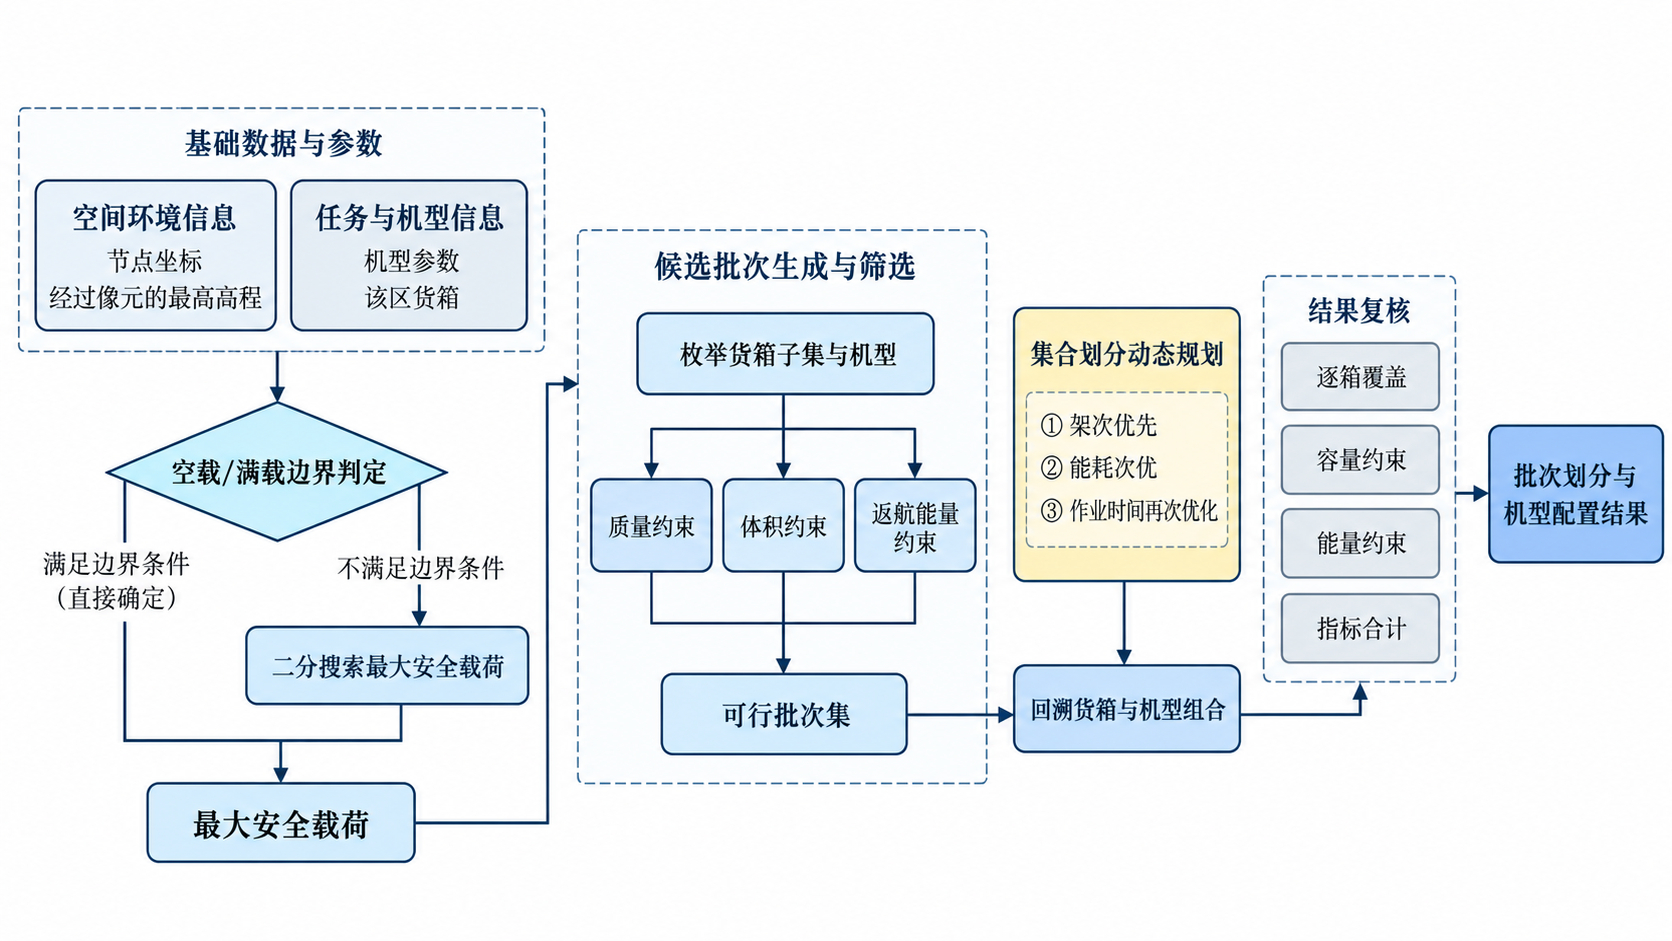
\includegraphics[width=\textwidth]{figures/q1/figure5.png}
\caption{单点运输能力与货箱组批求解流程}\label{fig:q1-flow}
\end{figure}

\subsection{安全载荷计算结果}
按修正后的DEM穿越像元口径，对15个服务区和3种机型共45个组合重新计算最大安全载荷，结果如图~\ref{fig:q1-safe-payload}所示。45个组合均可完成空载返航，其中A型在全部服务区均达到25~kg额定载荷；B型仅在S008受能量约束，最大安全载荷为28.632~kg；C型在S002、S003、S004、S008和S012分别降至68.554、68.235、63.259、58.436和68.015~kg，其余服务区均达到80~kg额定载荷。S008--C的载荷保持率最低，为73.0\%。该图只呈现安全载荷的空间差异，差异由航程、沿途最高地形与机型载荷航程参数共同进入式~\eqref{eq:safe-payload}后产生。

\begin{figure}[H]
  \centering
  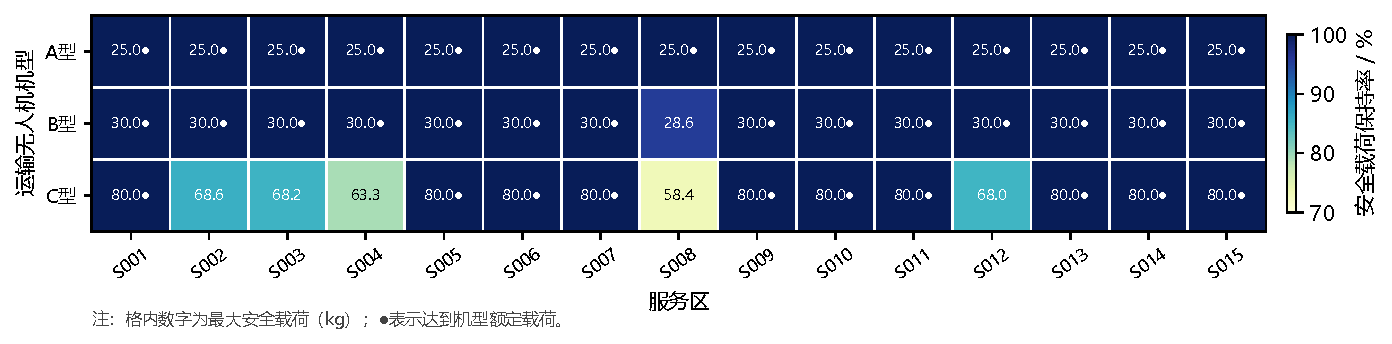
\includegraphics[width=\textwidth]{figures/q1/q1_safe_payload_heatmap.pdf}
  \caption{不同服务区与运输无人机机型的最大安全载荷}
  \label{fig:q1-safe-payload}
\end{figure}

\subsection{组批方案与结果分析}
将各服务区货箱分别代入集合划分动态规划后，80个货箱均被覆盖且恰好出现一次，不存在遗漏、重复或跨区组批。最终得到18个单点往返架次，其中B型与C型各承担9架次，A型未被选用；S001、S002和S003各需要2架次，其余12个服务区各需要1架次。全部架次的累计往返能耗为59.240~kWh，累计作业时间为9.111~h。这里的累计时间是各独立架次作业时长之和，不代表考虑实体机和共享电池后的调度完工时间，后者在问题二中计算。

\begin{table}[htbp]
  \centering
  \caption{问题一组批结果汇总}
  \label{tab:q1-summary}
  \begin{tabular}{lr}
    \toprule
    指标 & 计算结果 \\
    \midrule
    唯一覆盖货箱数 & 80箱 \\
    总架次数 & 18架次 \\
    A/B/C型架次数 & 0/9/9 \\
    累计往返能耗 & 59.240~kWh \\
    累计作业时间 & 9.111~h \\
    \bottomrule
  \end{tabular}
\end{table}

为判断各批次由哪类容量约束主导，定义质量、体积和安全可用能量利用率分别为
\begin{equation}
\eta_r^m=\frac{w_r}{Q_{g_r}},\qquad
\eta_r^v=\frac{v_r}{V_{g_r}},\qquad
\eta_r^e=\frac{E_r}{(1-\rho_{g_r})E_{g_r}^{use}}.
\end{equation}
图~\ref{fig:q1-utilization}给出18个批次的三类利用率。质量、体积和能量利用率的均值分别为78.7\%、77.2\%和68.4\%。若以三项利用率中的最大者作为该批次最紧约束，则9个批次最接近体积上限、5个最接近质量上限、4个最接近能量上限。Q1--S001--02的质量与体积利用率最高，分别为97.5\%和94.0\%；Q1--S004--01的能量利用率最高，达到96.5\%。这说明未达到额定载质量并不等于装载低效：完整货箱不可拆分，且部分批次会先触及舱容或安全能量边界。

\begin{figure}[H]
  \centering
  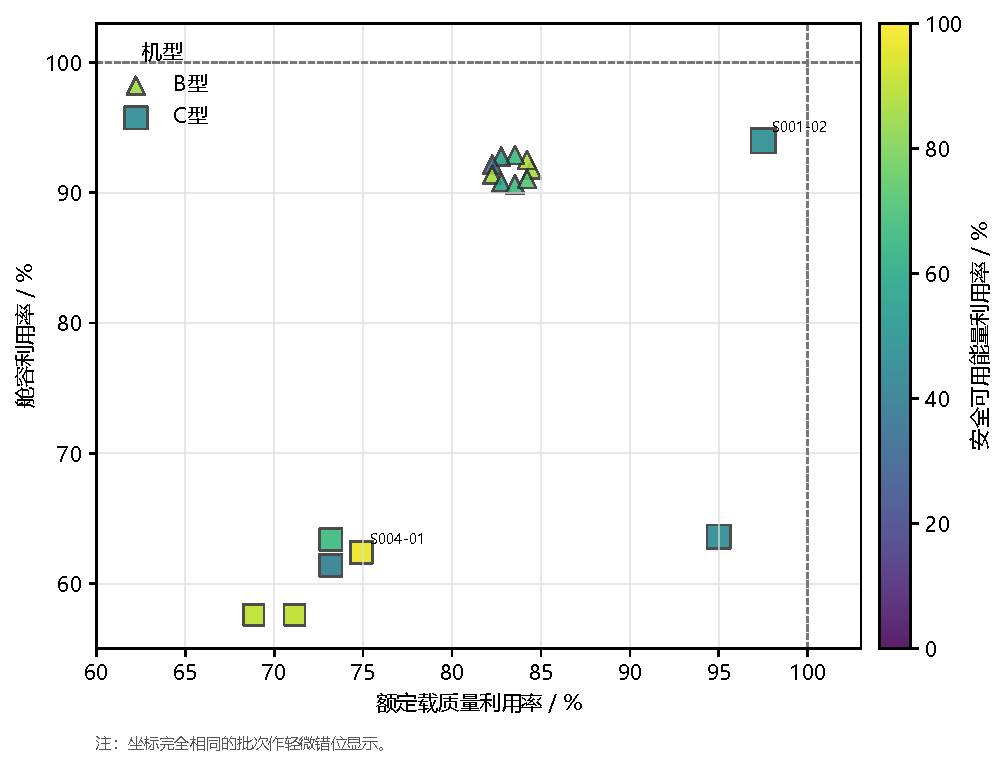
\includegraphics[width=0.82\textwidth]{figures/q1/q1_batch_utilization.pdf}
  \caption{问题一最终运输批次的质量、体积与能量利用率}
  \label{fig:q1-utilization}
\end{figure}

\section{问题二：异构无人机多点多架次运输调度}
\subsection{问题分析}
\subsubsection{由独立组批到耦合调度}
问题二取消“单服务区直接往返”的限制，允许一次飞行串访多个服务区，并要求明确实体无人机、电池和开始时刻。与问题一相比，新增自由度能够减少重复返航，却也引入三类耦合：访问顺序改变每箱交付时刻；前站卸货改变后续航段的剩余载荷和能耗；实体机与共享电池的再次可用时刻又决定任务能否并行。因而，问题二不是把问题一的18个批次简单排队，也不是普通的容量车辆路径问题。

题目中的医疗与首批保障要求具有硬约束性质，而一般物资的期望时间用于评价服务质量。若把两类时限放入同一个加权罚函数，算法可能用多个紧急箱迟到换取较短总路程，这与应急保障逻辑不符。因此本文先把硬违约数固定为0，再在可行集合内评价一般物资迟到、完工时间、能耗和架次数。

\subsubsection{关键决策与难点}
问题二需要同时确定六类决策：货箱属于哪个架次、同一架次访问哪些服务区、访问顺序如何、采用何种机型、分配哪架实体机与哪块同型电池、何时开始准备。前四类决定任务本身的持续时间和能耗，后两类决定任务能否在资源时间轴上落地。若只先求路线再任意分配资源，可能出现硬时限可行的抽象路线因电池尚未充满而无法按时起飞。

另一个难点是“到达”与“交付完成”不同。无人机抵达服务区后需要基础作业和逐箱交接，同站不同货箱的完成时刻并不相同；以到达时刻判断截止会系统性低估后排货箱的延误。本文保留站内交接顺序，并在每次卸货后更新剩余载荷，使时间和能量沿同一访问序列同步递推。

\subsubsection{求解框架选择}
完整问题同时含集合划分、异构车辆路径、时间窗和双资源排程，直接建立大规模混合整数模型会产生大量“货箱—架次—顺序—实体—电池—时刻”组合变量。考虑到题目规模和硬时限可行性的重要性，本文采用分层构造方法：分别建立硬箱专送基线与同目的地混装方案，对剩余软箱执行单区精确组批和异区双点串访合并，最后用事件仿真器分配实体机和满电电池。两套方案均重新计算完整物理量，不以距离近似替代能量和时限复核。

\subsection{时限—能量—资源统一模型}
\paragraph{决策表示与硬软时限}
将运输架次$r$表示为机型$g_r$、访问序列$\pi_r$、货箱集合$B_r$、实体机$u_r$、共享电池$k_r$及准备开始时刻$s_r$。每个货箱必须恰属于一个架次，并在自身目的服务区交付；机型与实体机、电池类型必须匹配。

对医疗箱和首批保障箱定义适用截止集合$\mathcal D_b$：医疗箱加入期望时刻，首批箱加入首批截止。硬时限箱满足
\begin{equation}d_b^{hard}=\min\mathcal D_b,\qquad C_b\le d_b^{hard}.\end{equation}
对$\mathcal D_b=\varnothing$的软时限箱，仅在目标中评价归一化加权迟到：
\begin{equation}
WTD=\sum_{b\in B^{soft}}\alpha_b\frac{\max(0,C_b-d_b^{exp})}{d_b^{exp}}.\label{eq:wtd}
\end{equation}
这里的“送达”采用完成该箱交接的时刻$C_b$，并非无人机到达服务区的时刻。这样的区分在同站多箱交接时会影响临界货箱是否逾期。

\paragraph{逐站时刻与剩余载荷递推}
令$\pi_r=(i_1,\ldots,i_m)$，$i_0=O01$，起飞时刻为
\begin{equation}\tau_{r0}^{dep}=s_r+t_{g_r}^{prep}+|B_r|t_{g_r}^{load}.\end{equation}
到达第$j$个服务区、完成站内投送和离开的时刻依次为
\begin{align}
\tau_{rj}^{arr}&=\tau_{r,j-1}^{dep}+t_{g_r,i_{j-1},i_j},\\
C_b&=\tau_{rj}^{arr}+t_{g_r}^{base}+\ell_b t_{g_r}^{handover},\\
\tau_{rj}^{dep}&=\tau_{rj}^{arr}+t_{g_r}^{base}+|B_{ri_j}|t_{g_r}^{handover}.
\end{align}
其中$\ell_b$为货箱在该站的交接序号。按有效硬截止升序、应急优先系数降序、编号升序排列，软时限箱在硬时限箱后依上述规则交接。离站后扣除本次交付质量，再用新的剩余载荷计算下一航段能耗。末站离开后加返航时间，得到$\tau_r^{ret}$。

这一递推把访问顺序同时作用于时间和能耗：较早卸下重箱可减轻后续载荷，但可能推迟其他节点的硬时限箱。多点路线必须逐段重算，不能仅在两个单点能耗之间做距离修正。

\paragraph{实体机与电池的双资源约束}
运输实体机在半开区间$[s_r,\tau_r^{ret})$被占用；电池还需完成返航后的充电，因此其占用区间为
\begin{equation}I_r^{bat}=[s_r,\tau_r^{ret}+T^{chg}(SOC_r^{end})).\end{equation}
对每个实体机$u$和电池$k$，同一时刻分别满足
\begin{equation}
\sum_{r:u_r=u}\ind_{[s_r,\tau_r^{ret})}(t)\le1,\qquad
\sum_{r:k_r=k}\ind_{I_r^{bat}}(t)\le1.
\end{equation}
半开区间使“上一任务结束的瞬间开始下一任务”不会被重复计为冲突。题面未另给运输机周转时长，实体机返回后可开始准备；其原电池仍在充电时，可以换用已经满电的同型电池。

图\ref{fig:q2-resource}用符号时刻说明两类资源的差异。机体可再次执行并不意味着原电池可再次使用；这也是仅按无人机架数排列甘特图不足以检验资源可行性的原因。
\begin{figure}[htbp]\centering
\begin{tikzpicture}[x=.8cm,y=1cm,font=\small]
\draw[edge](0,0)--(13,0) node[right]{时间};
\node[anchor=east] at(0,1.2){实体机};\node[anchor=east]at(0,2.3){电池};
\filldraw[fill=blue!12,draw=blue!50] (1,.8) rectangle (7,1.6);
\node at(4,1.2){准备、飞行、交付与返航};
\filldraw[fill=blue!12,draw=blue!50] (1,1.9) rectangle (7,2.7);
\filldraw[fill=orange!15,draw=orange!60] (7,1.9) rectangle (12,2.7);
\node at(4,2.3){执行任务};\node at(9.5,2.3){返航后充电};
\foreach \x in {1,7,12}{\draw[dashed,gray](\x,0)--(\x,2.8);}
\node[below]at(1,0){$s_r$};\node[below]at(7,0){$\tau_r^{ret}$};
\node[below]at(12,0){$\tau_r^{ret}+T^{chg}$};
\end{tikzpicture}
\caption{运输机与共享电池占用差异示意；横向长度不代表实际计算时长}\label{fig:q2-resource}
\end{figure}

\subsection{求解流程与指标权衡}
\paragraph{分层评价指标}
在全部硬约束成立的集合内，以$(WTD,C_{max},E_T,N_T)$作为分层比较指标，其中
\begin{equation}C_{max}=\max_r\tau_r^{ret},\quad E_T=\sum_rE_r,\quad N_T=|\mathcal R|.\end{equation}
先保证医疗与首批交付，再比较一般物资及时性；在及时性相同的候选中依次减少完工时间、能耗和架次数。该目标定义评价偏好，并不意味着构造算法已经穷尽其可行集合。

\paragraph{基线与混装方案构造}
求解先构造硬箱专送基线并确定紧迫批次的实体机指派，再据此形成同目的地混装方案：对各服务区枚举普通货箱补入组合，补入后的架次重新核验质量、体积、逐段递减载荷能耗、返航余量及每个硬时限，并保持硬时限箱优先交接。剩余货箱执行单服务区精确组批，随后把能够节能的两个异区单点任务贪心合并为双区串访。该构造吸收了带时间窗路径问题“先保证可行、再组合任务”的思想\textsuperscript{\cite{Ropke2006}}，但当前程序并未实现通用大邻域搜索。

两套方案均依次执行三项确定性操作：同目的地软箱补入、剩余软箱精确组批、异区单点任务节能合并；合并时比较两种访问顺序。随后分别完成实体资源排程，并按$(N_{late}^{hard},WTD,C_{max},E_T,N_T)$字典序比较整套结果。因程序只在这两套构造中择优，结论表述为“当前构造方案优于所列基线”，不宣称已搜索全部拆分与合并组合。

\paragraph{事件仿真与资源落地}
对每种机型分别维护实体机可用时刻$a_u$和电池满电时刻$a_k$。当一个抽象运输任务$r$进入排程时，枚举同型实体机—电池组合，其最早准备开始时刻为
\begin{equation}
s_r(u,k)=\max\{a_u,a_k,r_r^{release}\},
\end{equation}
其中$r_r^{release}$表示由硬截止逆推或波次约束给出的最早释放要求。将$s_r(u,k)$代入完整路线递推，得到逐箱交付、返航SOC与充电结束时刻；对容量和能量可行的组合，按硬迟到箱数、最大硬迟到、软时限代价、交付时刻、能耗和资源恢复时刻依次评分，然后更新$a_u$和$a_k$。这一过程把“选哪个任务”与“任务何时能够真实执行”分开处理；最终方案再统一核验硬迟到为0。

事件仿真的核心步骤为：
\begin{enumerate}
  \item 按硬截止、任务紧迫度和候选增量代价选择下一待排任务；
  \item 枚举同型实体机与电池，计算最早可开始时刻；
  \item 逐站递推到达、交付、离开、返航、SOC和充电完成；
  \item 容量或返航余量不可行的组合不进入评分；对其余组合计算硬迟到、软迟到及资源恢复指标；
  \item 接受评分最小的组合，写入任务、交付和资源事件表，并在最终方案核验硬迟到为0；
  \item 所有任务完成后执行覆盖守恒与区间冲突扫描。
\end{enumerate}

图~\ref{fig:q2-flow}给出问题二从货箱分层到资源事件审计的完整流程。容量或能量检查不通过的路线不进入资源评分；硬时限偏差则作为评分的最高优先级，并在整套方案形成后再次核验。
\begin{figure}[H]\centering
\begin{tikzpicture}[node distance=6mm]
\node[block,text width=7.4cm](input){读取货箱、机型、实体机、电池与DEM\\划分硬时限箱和软时限箱};
\node[block,text width=7.4cm,below=of input](seed){构造硬箱专送基线\\确定紧迫任务与实体机指派};
\node[block,text width=7.4cm,below=of seed](mix){枚举软箱补入、单区组批与双区串访\\逐站更新剩余载荷和交付时刻};
\node[block,text width=7.4cm,below=of mix](feas){检查质量、体积、DEM净空、返航SOC与硬时限};
\node[block,text width=7.4cm,below=of feas](event){事件仿真分配实体机与满电电池\\传播返航、充电和再次可用时刻};
\node[block,text width=7.4cm,below=of event](select){与硬箱专送基线按字典序比较\\输出路线、逐箱交付与资源时间轴};
\draw[edge](input)--(seed);\draw[edge](seed)--(mix);\draw[edge](mix)--(feas);
\draw[edge](feas)--node[right,font=\small]{通过}(event);\draw[edge](event)--(select);
\draw[edge](feas.east)--++(1.1,0) node[right,font=\small]{不通过} |- (mix.east);
\end{tikzpicture}
\caption{问题二异构运输调度求解流程}\label{fig:q2-flow}
\end{figure}

\subsection{调度结果与对比分析}
\paragraph{基线设置与总体指标}
基于修正后的DEM穿越像元高程口径，表~\ref{tab:q2-compare}给出两套构造方案的实算比较。两者均完成80箱唯一交付，31箱硬时限货箱均无违约；混装方案把普通物资超期箱数由23箱降至9箱，并同时减少架次、完成时间和能耗，故选作问题二当前方案。
\begin{table}[htbp]
  \centering
  \caption{问题二基线与硬软混装方案比较}
  \label{tab:q2-compare}
  \begin{tabular}{lrrrrrr}
    \toprule
    方案 & 硬违约/箱 & 普通超期/箱 & $WTD$ & $C_{max}$/h & $E_T$/kWh & 架次 \\
    \midrule
    硬箱专送基线 & 0 & 23 & 111.492 & 3.527 & 83.012 & 26 \\
    硬软混装方案 & 0 & 9 & 38.787 & 2.679 & 69.602 & 22 \\
    \bottomrule
  \end{tabular}
\end{table}

\paragraph{资源时间轴与可执行性}
图~\ref{fig:q2-gantt}进一步给出所选22架次在8架实体运输机和14块共享电池上的实际占用区间。上图浅色段为起飞前准备与装载，深色段为起飞至返航；下图彩色段为电池执行任务，灰色段为返航后的两阶段充电。任一实体机的任务区间均不重叠，同一电池的新任务也均在上一充电区间结束后开始。全部运输机于2.679~h前返航，最后一块电池于3.386~h完成充电，因此运输完工时间与资源完全恢复时间应分别报告。

\begin{figure}[H]
  \centering
  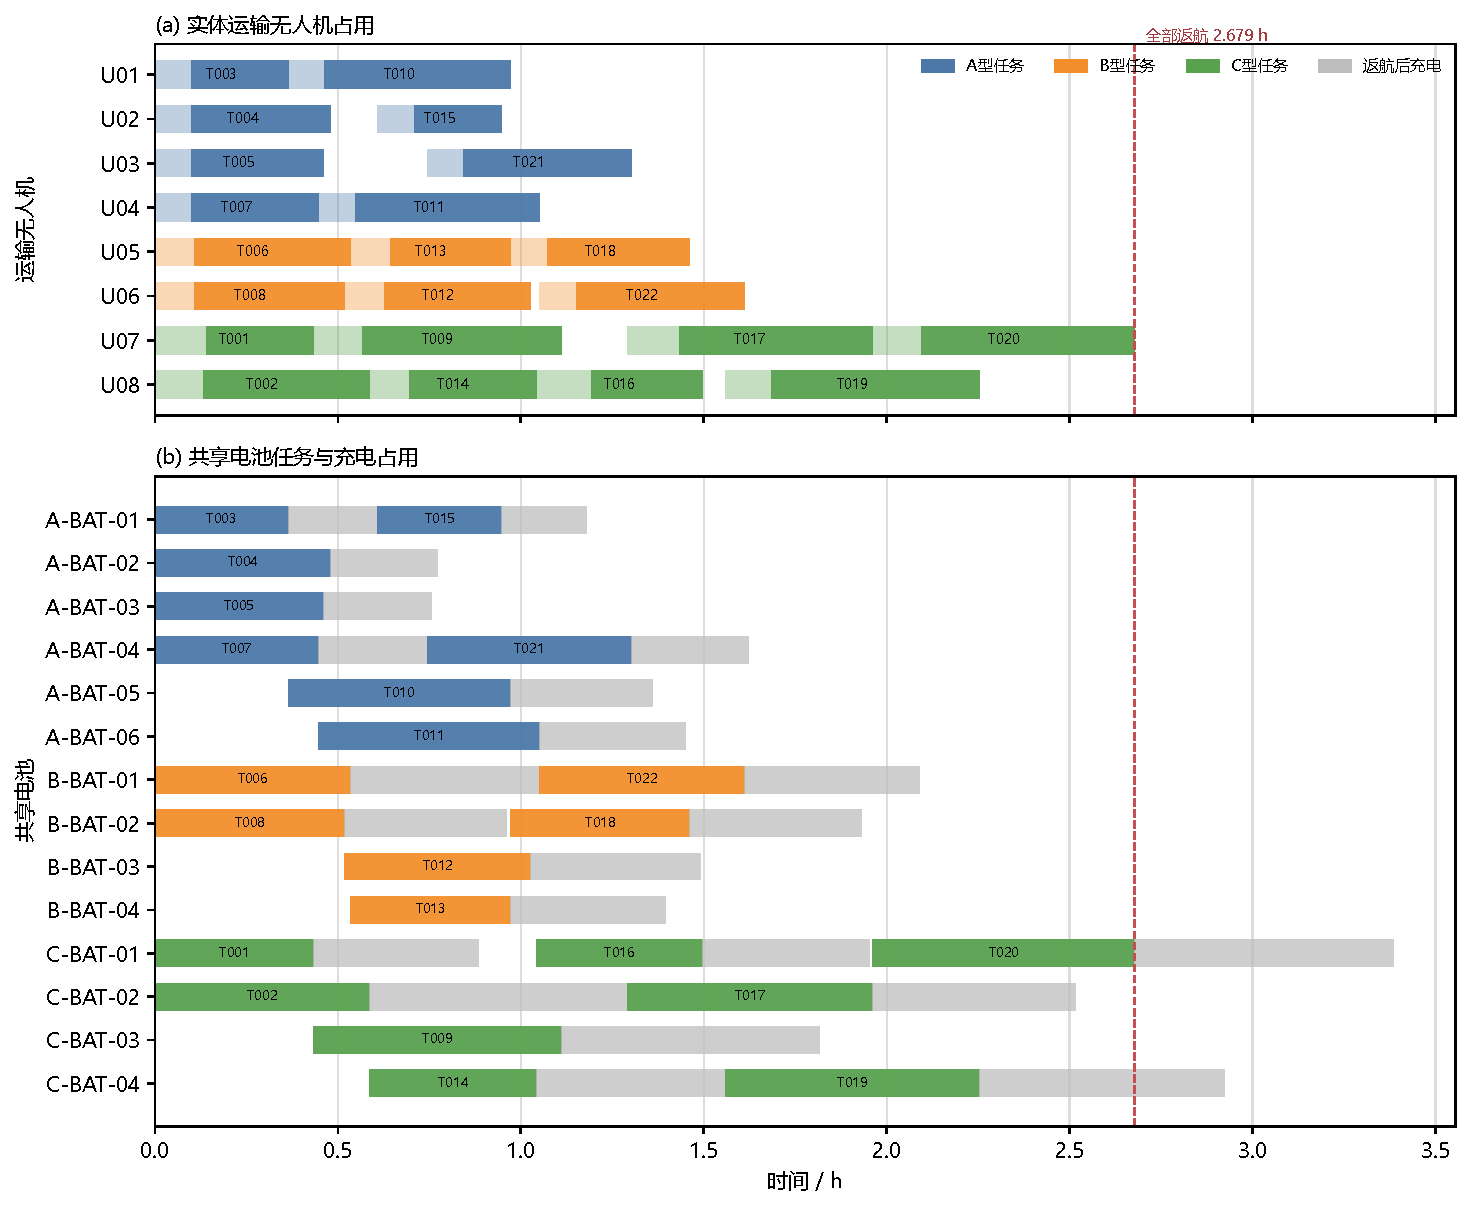
\includegraphics[width=\textwidth]{figures/q2/q2_resource_gantt.pdf}
  \caption{问题二运输无人机与共享电池联合甘特图。浅色段表示起飞前准备与装载，彩色段表示任务占用，灰色段表示返航后充电，红色虚线为全部运输架次返航完成时刻。}
  \label{fig:q2-gantt}
\end{figure}

\paragraph{改进幅度及其原因}
相对基线，混装方案的$WTD$下降65.2\%，全部返航完成时间缩短24.1\%，总运输能耗下降16.2\%，架次下降15.4\%。

四项指标同步改善的主要原因不是提高飞行速度，而是减少重复的准备、装载、爬升、返航和基础交接过程。把目的地相同的软箱补入已有紧急任务，可利用原本闲置的质量与体积；少量双区串访则在硬时限允许时减少一次完整往返。与此同时，方案仍有9个一般物资箱超过期望时刻，说明硬截止优先会把有限的早期机体与满电电池配置给紧急箱。该权衡是目标层次的直接结果，而不是程序漏排。

需要强调的是，22架次大于问题一的18架次并不矛盾。问题一允许各服务区独立比较组批，累计时间也不受实体资源和时限约束；问题二必须为31个硬时限箱保留早期交付能力，并在8架实体机和14块共享电池上形成真实时序。两问目标和约束不同，问题一用于能力下界与候选生成，问题二才回答标准场景下的可执行调度。

\section{问题三：连续通信约束下的运输与中继协同}
\subsection{问题分析}
\subsubsection{问题二与问题三的依赖关系}
问题三在运输可行性的基础上增加“任务全过程保持通信”的要求。通信需求不是服务区上的静态属性，而是随运输无人机位置和时间变化的轨迹属性；中继无人机也不是固定基站，它需要提前准备、飞抵候选点、完成建链，并在运输任务结束后返航和补能。因此，问题二提供的组批与路线只能作为运输侧候选，只有加入中继可达性、在位时段和资源周转后，才能判断联合方案是否真正可执行。

本文保留问题二的22条路线作为已通过硬时限与能量验证的候选，并在该候选上调整开始时刻、组织波次和配置中继。这样做能够清楚分离“运输方案本身是否可行”和“为了连续通信需付出多少等待与能量代价”，也便于沿用80箱唯一覆盖证据。相应局限是没有重新枚举所有组批、访问顺序和机型组合，因此所得结果是联合可行方案和当前搜索范围内的上界，而不是原问题完整联合决策空间中的全局最优解。

\subsubsection{时空耦合与主要难点}
连续通信至少包含四个层次。第一，链路必须双向可用，控制指令下发与状态回传任一方向不足都不能视为可通信；第二，地形遮挡只增加附加损耗，是否中断仍需与链路预算比较；第三，中继模式要求“运输机—中继”和“中继—网关”两条链路在同一时刻同时成立；第四，运输轨迹上的每一时刻都必须被直连或某架实际在服中继覆盖。

其计算难点在于，离散采样点全部可用并不能排除相邻样本之间的短时断链。山地视线关系还可能在航段经过像元边界时发生变化，使传播损耗并非仅由端点距离决定。故本文把固定步长采样用于候选筛选和独立复核，最终可行性由连续区间证书判断。

\subsubsection{输出目标与评价次序}
联合方案需要输出运输开始时刻、中继悬停点与服务区间、实体中继机和能源组件、每段通信方式、联合完成时间及总能耗。评价时首先要求31个硬时限箱不违约、每条运输轨迹连续通信、各类资源区间不冲突；在此基础上再比较一般物资迟到、联合完成时间、中继能耗和中继架次数。最小链路余量作为稳健性诊断指标单独报告，不用平均余量掩盖局部薄弱点。

\subsection{通信可用性模型}
\paragraph{双向链路预算}
固定网关G01位于O01，通信端点海拔由地面海拔与天线离地高度确定；运输端点随爬升、巡航、下降和交接阶段变化。接收门限为灵敏度与衰落裕量之和，附件中相应值为
\begin{equation}P_{th}=P_{sens}+M=-98+8=-90\ \mathrm{dBm}.\end{equation}
对通信方向$a\to b$，允许传播损耗为
\begin{equation}
L_{a\to b}^{max}=P_t^a+G_t^a+G_r^b-L_{sys}-P_{th}^b,\qquad
L_{ab}^{max}=\min(L_{a\to b}^{max},L_{b\to a}^{max}).
\end{equation}
两个方向取小值，是因为指令下发与状态回传均须可用。将附件对应接口参数代入，可得运输机—网关、运输机—中继和中继—网关的双向预算分别为122、116和126 dB。这些是设备参数推导的门限，不是某条实际航迹的通信余量。

设$D_{ab}(t)$为端点三维直线距离，单位km；频率$f$以MHz计，附件2.4 GHz对应2400 MHz。自由空间损耗常数及单位换算采用ITU-R P.525口径\textsuperscript{\cite{ITUP525}}；山地空地链路还需显式考虑视距与地形遮挡\textsuperscript{\cite{Feng2006,Zeng2016}}。传播损耗为
\begin{equation}
L_{ab}^{path}(t)=32.45+20\log_{10}f+20\log_{10}D_{ab}(t)+L_{obs}\beta_{abt}.
\end{equation}
其中$L_{obs}=10$ dB，遮挡变量由三维视线与沿途DEM比较确定。系统损耗已在预算侧扣除，不能在传播损耗侧再次扣减。定义
\begin{equation}
A_{ab}(t)=\ind\{L_{ab}^{path}(t)\le L_{ab}^{max}\},\quad
M_{ab}^{link}(t)=L_{ab}^{max}-L_{ab}^{path}(t).
\end{equation}
遮挡增加损耗，但不必然导致链路中断；最终仍须比较预算门限。

\paragraph{合法拓扑与全时段服务}
图\ref{fig:q3-topology}给出题目允许的两种通信方式。直连不可用时，可以经同一架中继完成接入和回传，不允许通过多架中继接力跳转。
\begin{figure}[htbp]\centering
\begin{tikzpicture}
\node[block,text width=2.5cm] (t) at(0,0){运输无人机};
\node[block,text width=2.5cm] (r) at(5,0){在服中继};
\node[block,text width=2.5cm] (g) at(10,0){固定网关G01};
\draw[edge,<->](t)--node[above,font=\small]{接入链路}(r);
\draw[edge,<->](r)--node[above,font=\small]{回传链路}(g);
\draw[edge,<->](t.south)--++(0,-1.1)--node[below,font=\small]{直连链路}(10,-1.6)--(g.south);
\node[font=\small,align=center] at(5,1.4){中继模式要求接入与回传同时可用\\拓扑示意，不表示实际点位或覆盖范围};
\end{tikzpicture}
\caption{直连与单中继通信拓扑示意}\label{fig:q3-topology}
\end{figure}

令$\mathcal T_r$为运输架次需要保障的全部飞行与交接时刻，$I_h^{srv}$为中继$h$的在服区间。对任意$t\in\mathcal T_r$，要求
\begin{equation}
A_{rG}(t)=1\quad\text{或}\quad
\exists h:\ t\in I_h^{srv},\ A_{rh}(t)=1,\ A_{hG}(t)=1.
\label{eq:continuous}
\end{equation}
输出时优先标记直连；非直连时选择一架满足条件的中继，保证每时刻只有一个实际保障指派。允许多个中继在物理上可用，但不能由此把同一运输区间同时计作多项必要保障任务。

\subsection{中继任务与资源模型}
\paragraph{候选悬停点与飞行过程}
候选悬停点$p$须在DEM内，海拔为$H_p^R=H_p^{DEM}+h_p^{AGL}$，且$0<h_p^{AGL}\le300$ m。中继出航巡航海拔还要覆盖终点悬停海拔：
\begin{equation}
H_{O01,p}^{c}=\max\left(\max_{c\in\mathcal C_{O01,p}}H_c+50,\ H_p^R\right).
\end{equation}
出航按爬升、水平巡航、必要下降计算，返航同理。中继从准备开始到建链完成的时刻依次为
\begin{align}
\tau_h^{dep}&=s_h+t_R^{prep},&
\tau_h^{arr}&=\tau_h^{dep}+t_{O01,p}^{fly},\\
\tau_h^{link}&=\tau_h^{arr}+t_R^{link},&
\tau_h^{ret}&=\tau_h^{end}+t_{p,O01}^{fly}.
\end{align}
只有在$[\tau_h^{link},\tau_h^{end}]$内才能提供保障。总能耗写为
\begin{align}
E_h^{fly}&=\frac{P_R^{cr}}{3600}\left(\frac{d_{O01,p}}{v_R^{cr}}+\frac{d_{p,O01}}{v_R^{cr}}\right)
+\frac{m_Rg_0(h_{O01,p}^{+}+h_{p,O01}^{+})}{3.6\times10^6\eta_R^{up}},\\
E_h&=E_h^{fly}+\frac{(P_R^{hover}+P_R^{com})(\tau_h^{end}-\tau_h^{arr})}{3600}
\le(1-\rho_R)E_R^{use}.\label{eq:relay-energy}
\end{align}
功率以kW计，故时间需除以3600。这里把建链期间按悬停及通信功率计入能源消耗，明确计费从抵达开始，而服务可用从建链完成开始。

\paragraph{实体机、能源组件与可用区间}
中继实体机占用$[s_h,\tau_h^{ret}+t_R^{turn})$；能源组件占用任务及返航后充电区间。两架中继机和六组能源组件均按实体编号分配，在同一波次内也须逐一预占，不能让多个任务同时选中尚未更新状态的同一资源。

\subsection{候选覆盖与联合调度方法}
\paragraph{离线选点与方案固化}
先将运输任务展开为分段线性三维轨迹，识别直连不足的时空位置。独立选点脚本在服务区邻域、航段附近和DEM高点形成候选悬停集合，并按5~s黑障样本筛选越界、回传不足和往返能量不可行的点。搜索得到的六个点位与七个运输波次随后固化到主求解器；离散样本仅用于离线筛选，最终仍按式\eqref{eq:continuous}验证整段时间。

离线候选点生成兼顾覆盖与代价。服务区邻域点有利于保障下降和交接阶段，航段投影附近点有利于缩短运输机—中继距离，局部高点则有利于改善中继—网关视距。对于每个候选点，先检查DEM范围和离地高度，再检查中继到网关的回传预算，最后计算出航、返航和最长可悬停时间。主求解器只接收离线筛选后固定的P1A、P1B、P2A、P2B、P3A和P4B六个点位，并显式检查输入是否为22个运输架次。

\paragraph{覆盖关系与运输波次}
将每条运输轨迹划分为直连区间和需要中继的区间。离线搜索把22个运输任务组织为W1--W7七个固定波次，并为每个波次配置一个或两个上述点位；中继须在波次首个需求时刻之前完成建链，并持续到最后一个实际保障区间结束。主程序依次执行这些固定波次，由资源事件仿真分配两架中继机和六套能源组件，再对全部链路实施连续认证。故该程序证明的是固化方案可行，而非在线贪心选点的全局最优性。

运输波次并非越集中越好。集中可以提高一次中继在位期间的覆盖利用率，但也可能需要多个中继点同时在服，并推迟部分运输任务；分散则降低并发资源，却增加重复准备、飞抵和返航。本文在硬时限和连续覆盖成立的前提下，以一般物资迟到、联合完成时间、能耗和架次数依次评价这种取舍。

图~\ref{fig:q3-flow}概括问题三的覆盖筛选、资源排程与连续认证闭环。离散样本只负责加速候选筛选；任何未通过连续区间认证的方案都必须返回选点或波次调整步骤。
\begin{figure}[H]\centering
\begin{tikzpicture}[node distance=6mm]
\node[block,text width=7.6cm](traj){读取运输路线与时序\\展开爬升、巡航、下降和交接轨迹};
\node[block,text width=7.6cm,below=of traj](blind){计算直连状态\\提取非直连时空区间};
\node[block,text width=7.6cm,below=of blind](candidate){读取离线筛选的六个悬停点\\核验点位、回传和往返能量};
\node[block,text width=7.6cm,below=of candidate](cover){执行固化的W1--W7运输波次\\分配中继机与能源组件};
\node[block,text width=7.6cm,below=of cover](cert){连续区间证书与0.5~s加密采样\\复核链路、能量和资源占用};
\node[block,text width=7.6cm,below=of cert](output){输出联合时序、通信分段、链路余量\\联合完工时间与总能耗};
\draw[edge](traj)--(blind);\draw[edge](blind)--(candidate);\draw[edge](candidate)--(cover);
\draw[edge](cover)--(cert);\draw[edge](cert)--node[right,font=\small]{通过}(output);
\draw[edge](cert.east)--++(1.2,0) node[right,font=\small]{未通过} |- (candidate.east);
\end{tikzpicture}
\caption{问题三运输—中继协同求解与认证流程}\label{fig:q3-flow}
\end{figure}

\paragraph{中继任务阶段与联合目标}
图\ref{fig:q3-phase}把最终选中的11个中继架次拆为准备、飞抵与建链、在位保障以及返航三个阶段。不同架次的在位时长差异明显，因此各架次均按实际保障区间核算能耗和资源占用。
\begin{figure}[htbp]
  \centering
  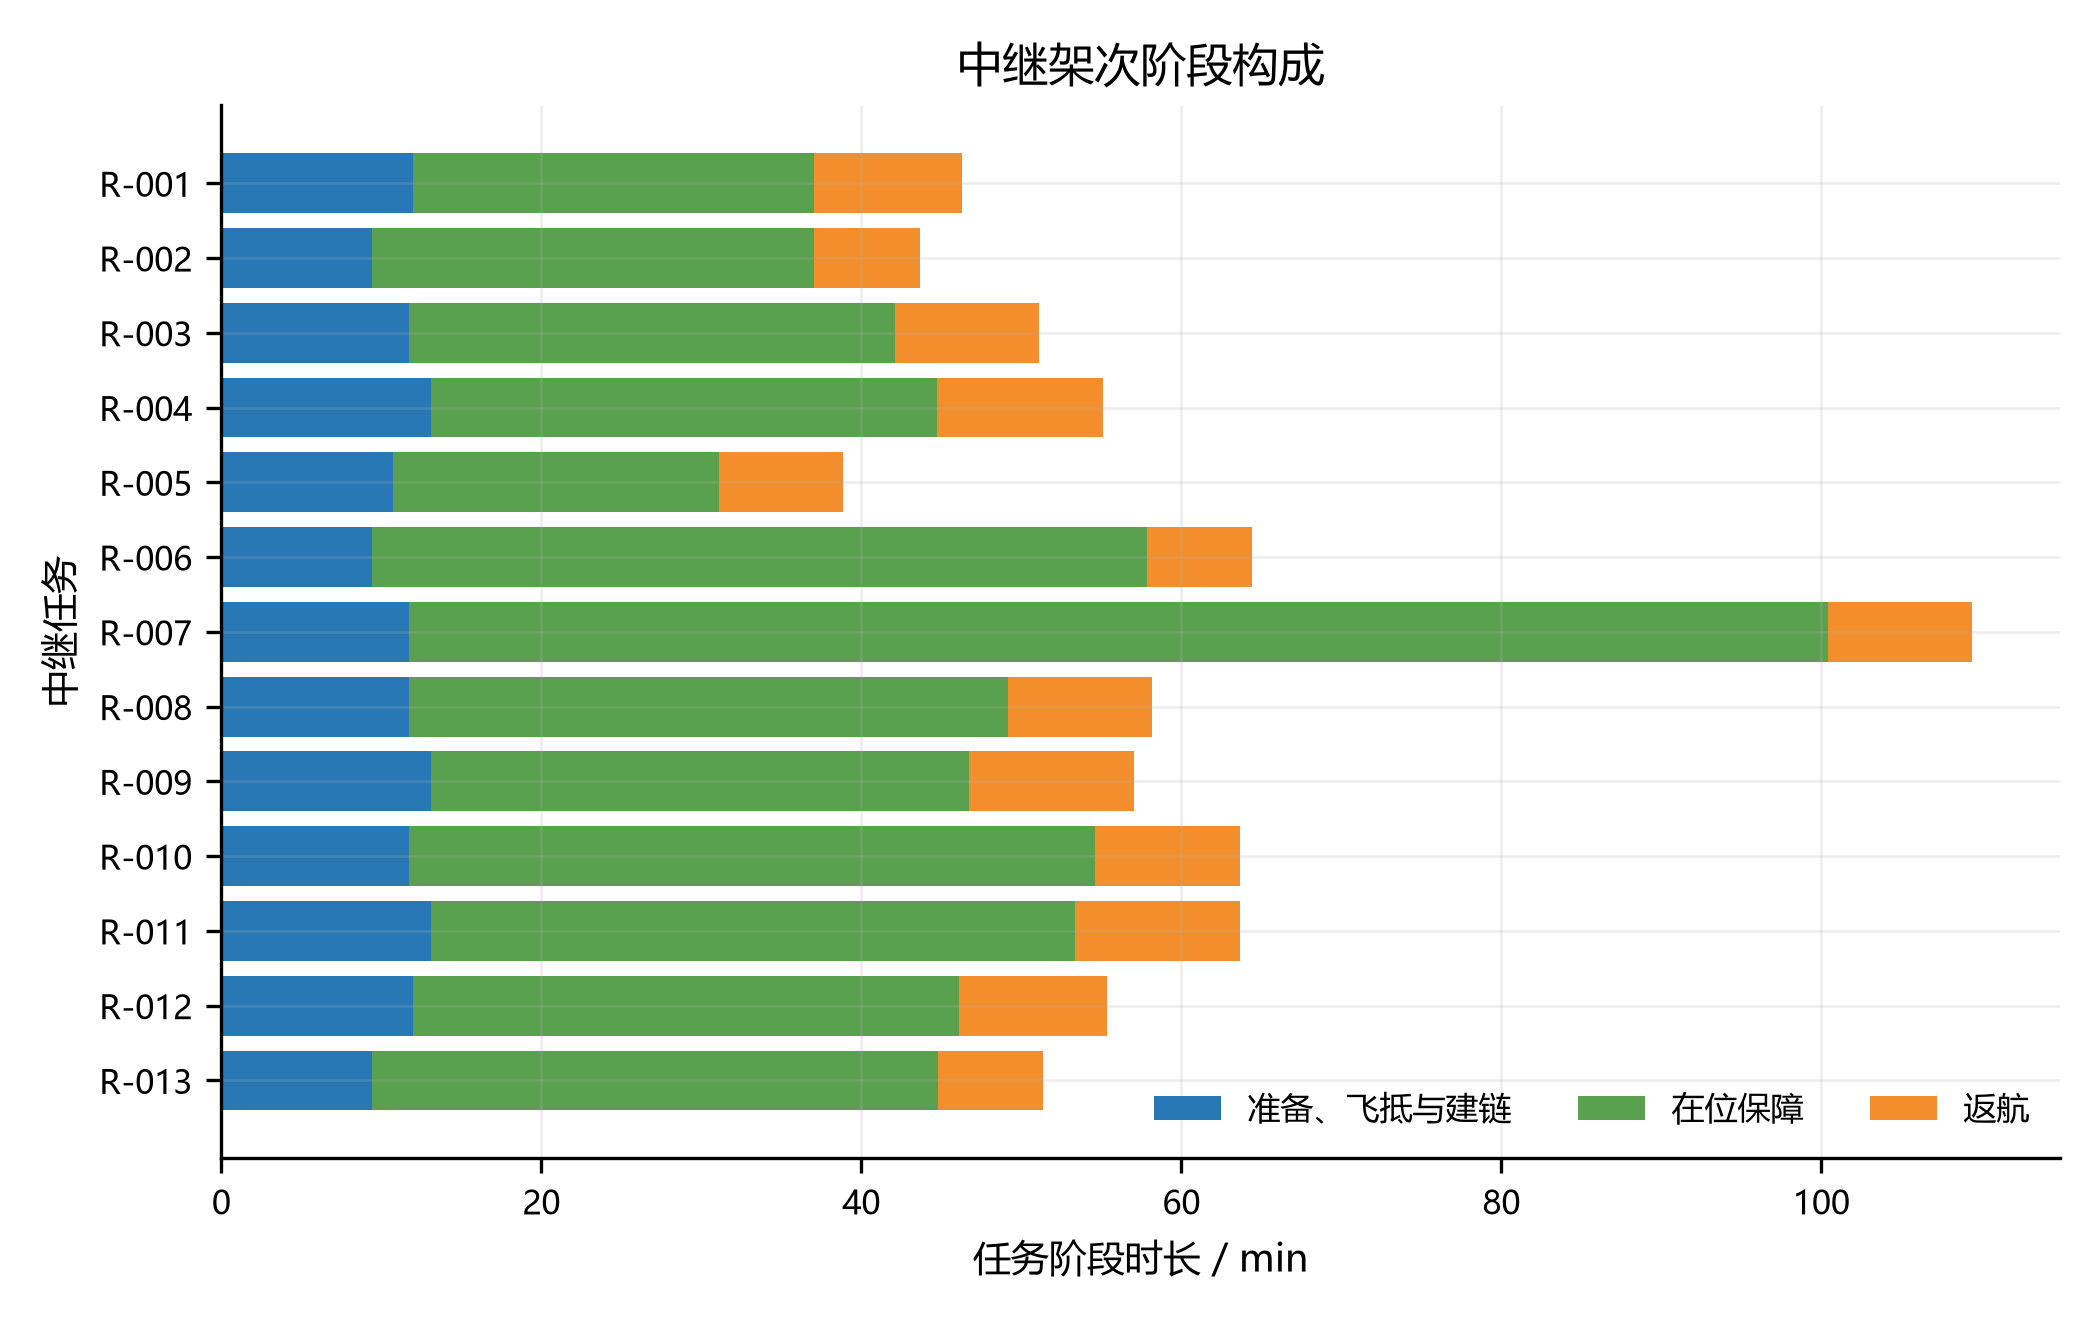
\includegraphics[width=0.92\textwidth]{figures/q3_q4/raw_q3_relay_phase_duration.png}
  \caption{中继架次的阶段时长构成}
  \label{fig:q3-phase}
\end{figure}

联合候选方案采用硬截止优先组织运输批次，并根据中继最早建链时刻、最长可服务时长和能源再可用时刻调整波次。比较指标为一般物资迟到、联合完成时间、总能耗和总架次，其中
\begin{equation}
C_{max}^{joint}=\max\!\left(\max_r\tau_r^{ret},\max_h\tau_h^{ret}\right),\quad
E^{joint}=\sum_rE_r+\sum_hE_h.
\end{equation}
完成时间取最后返航，不包含此后的充电及周转。硬时限与连续通信必须先满足；不能用较少的中继能耗补偿已发生的通信中断。

\subsection{连续性验证与联合调度结果}
\paragraph{连续区间认证方法}
固定时间网格不能排除相邻样本之间的短时中断。验证时，应在每个线性运动区间给出传播损耗上界：距离项在区间端点求上界，地形项采用扫掠视线与经过像元的关系获得保守判定；无法判定的区间进一步细分。区间达到细分阈值仍未被证明可用时，应标记为未通过证明，不将其自动视为可行，也不直接断言实际已经中断。

具体而言，先以轨迹的运动阶段端点、通信方式切换时刻和中继服务边界切分时间轴，使每个初始区间内端点运动均为线性。对直连候选，计算运输机到网关的距离上界和遮挡保守值；对中继候选，分别计算接入链路与回传链路的下界余量，并取二者较小值。若整个区间的服务余量下界非负，则该区间被认证；否则对半分割，直至找到可用证据或达到0.1~s阈值。达到阈值仍无法证明的区间按不可用处理，这一规则宁可拒绝边界方案，也不把数值不确定性误判为连续通信。

\paragraph{联合排程总体结果}
基于问题二的22条冻结路线，将任务按资源可行性和通信需求组织为7个波次。最终安排11个中继架次，使用2架中继无人机和5套能源组件，第6套能源组件保留备用。运输路线和运输能耗保持不变；为等待中继完成准备、飞抵和建链，运输完成时刻由问题二的$9643.106\ \mathrm{s}$延后到$23117.362\ \mathrm{s}$。最后一架中继于$23658.349\ \mathrm{s}$返航，因此联合完成时间为$6.572\ \mathrm{h}$。

\begin{table}[htbp]
  \centering
  \caption{问题三联合调度与连续通信的关键结果}
  \label{tab:q3-summary}
  \begin{tabular}{lrl}
    \toprule
    指标 & 数值 & 说明 \\
    \midrule
    运输架次/波次 & $22/7$ & 7个波次均配置中继 \\
    中继架次 & $11$ & 由2架中继机执行 \\
    实际使用能源组件 & $5$ & 库存为6套 \\
    通信分段数 & $68$ & 41段直连、27段中继 \\
    连续未解析区间 & $0$ & 22个架次均完成区间认证 \\
    0.5 s网格点/中断点 & $65532/0$ & 独立加密采样复核 \\
    最小保守链路余量 & $0.139703\ \mathrm{dB}$ & 出现在T005与T021 \\
    联合完成时间 & $23658.349\ \mathrm{s}$ & 取最后运输或中继返航 \\
    \bottomrule
  \end{tabular}
\end{table}

\paragraph{通信分段与双重验证}
连续区间证书把每段最小服务余量写为
\begin{equation}
M^{service}(t)=\max\left\{M_{TG}(t),\max_h\min\left[M_{TR_h}(t),M_{R_hG}(t)\right]\right\}.
\end{equation}
若采样余量减去区间变化上界后仍非负，则整段得到认证；否则继续二分。22个架次均未出现未解析区间；另以0.5 s步长检查65532个点，也未发现中断。表\ref{tab:q3-summary}汇总了连续区间认证与加密采样的结果。

图\ref{fig:q3-gantt}显示两架中继机在各波次之间交替执行，不存在机体占用重叠；能源组件的充电与复用由同一事件时间轴核算。图\ref{fig:q3-timeline}把68个通信分段展开，其中斜线区段表示实际使用中继。
\begin{figure}[htbp]
  \centering
  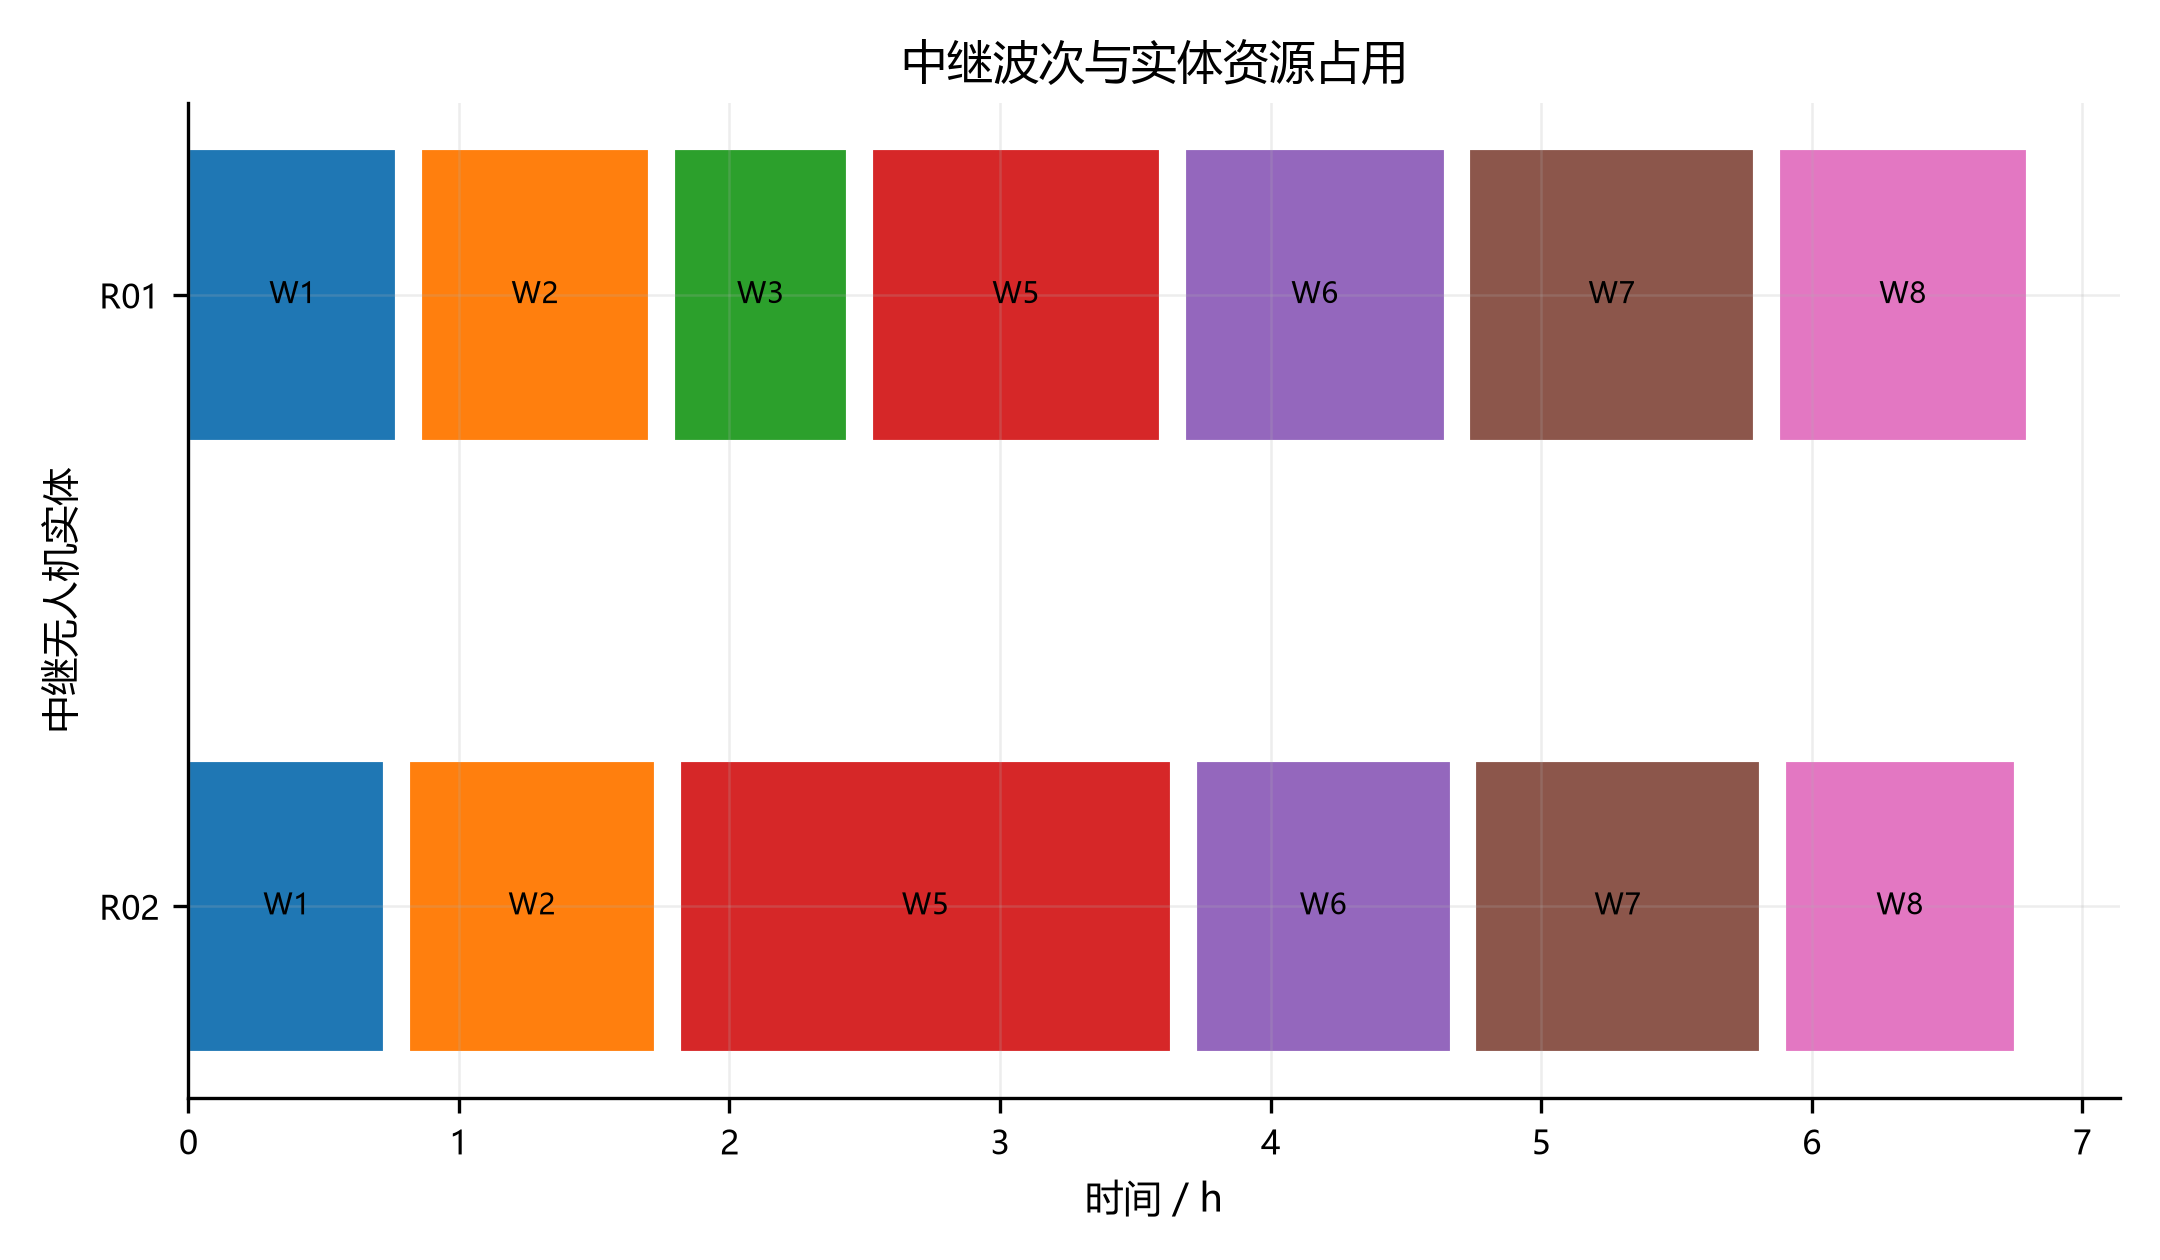
\includegraphics[width=0.92\textwidth]{figures/q3_q4/process_q3_relay_gantt.png}
  \caption{中继波次与实体资源占用时间轴}
  \label{fig:q3-gantt}
\end{figure}

\begin{figure}[htbp]
  \centering
  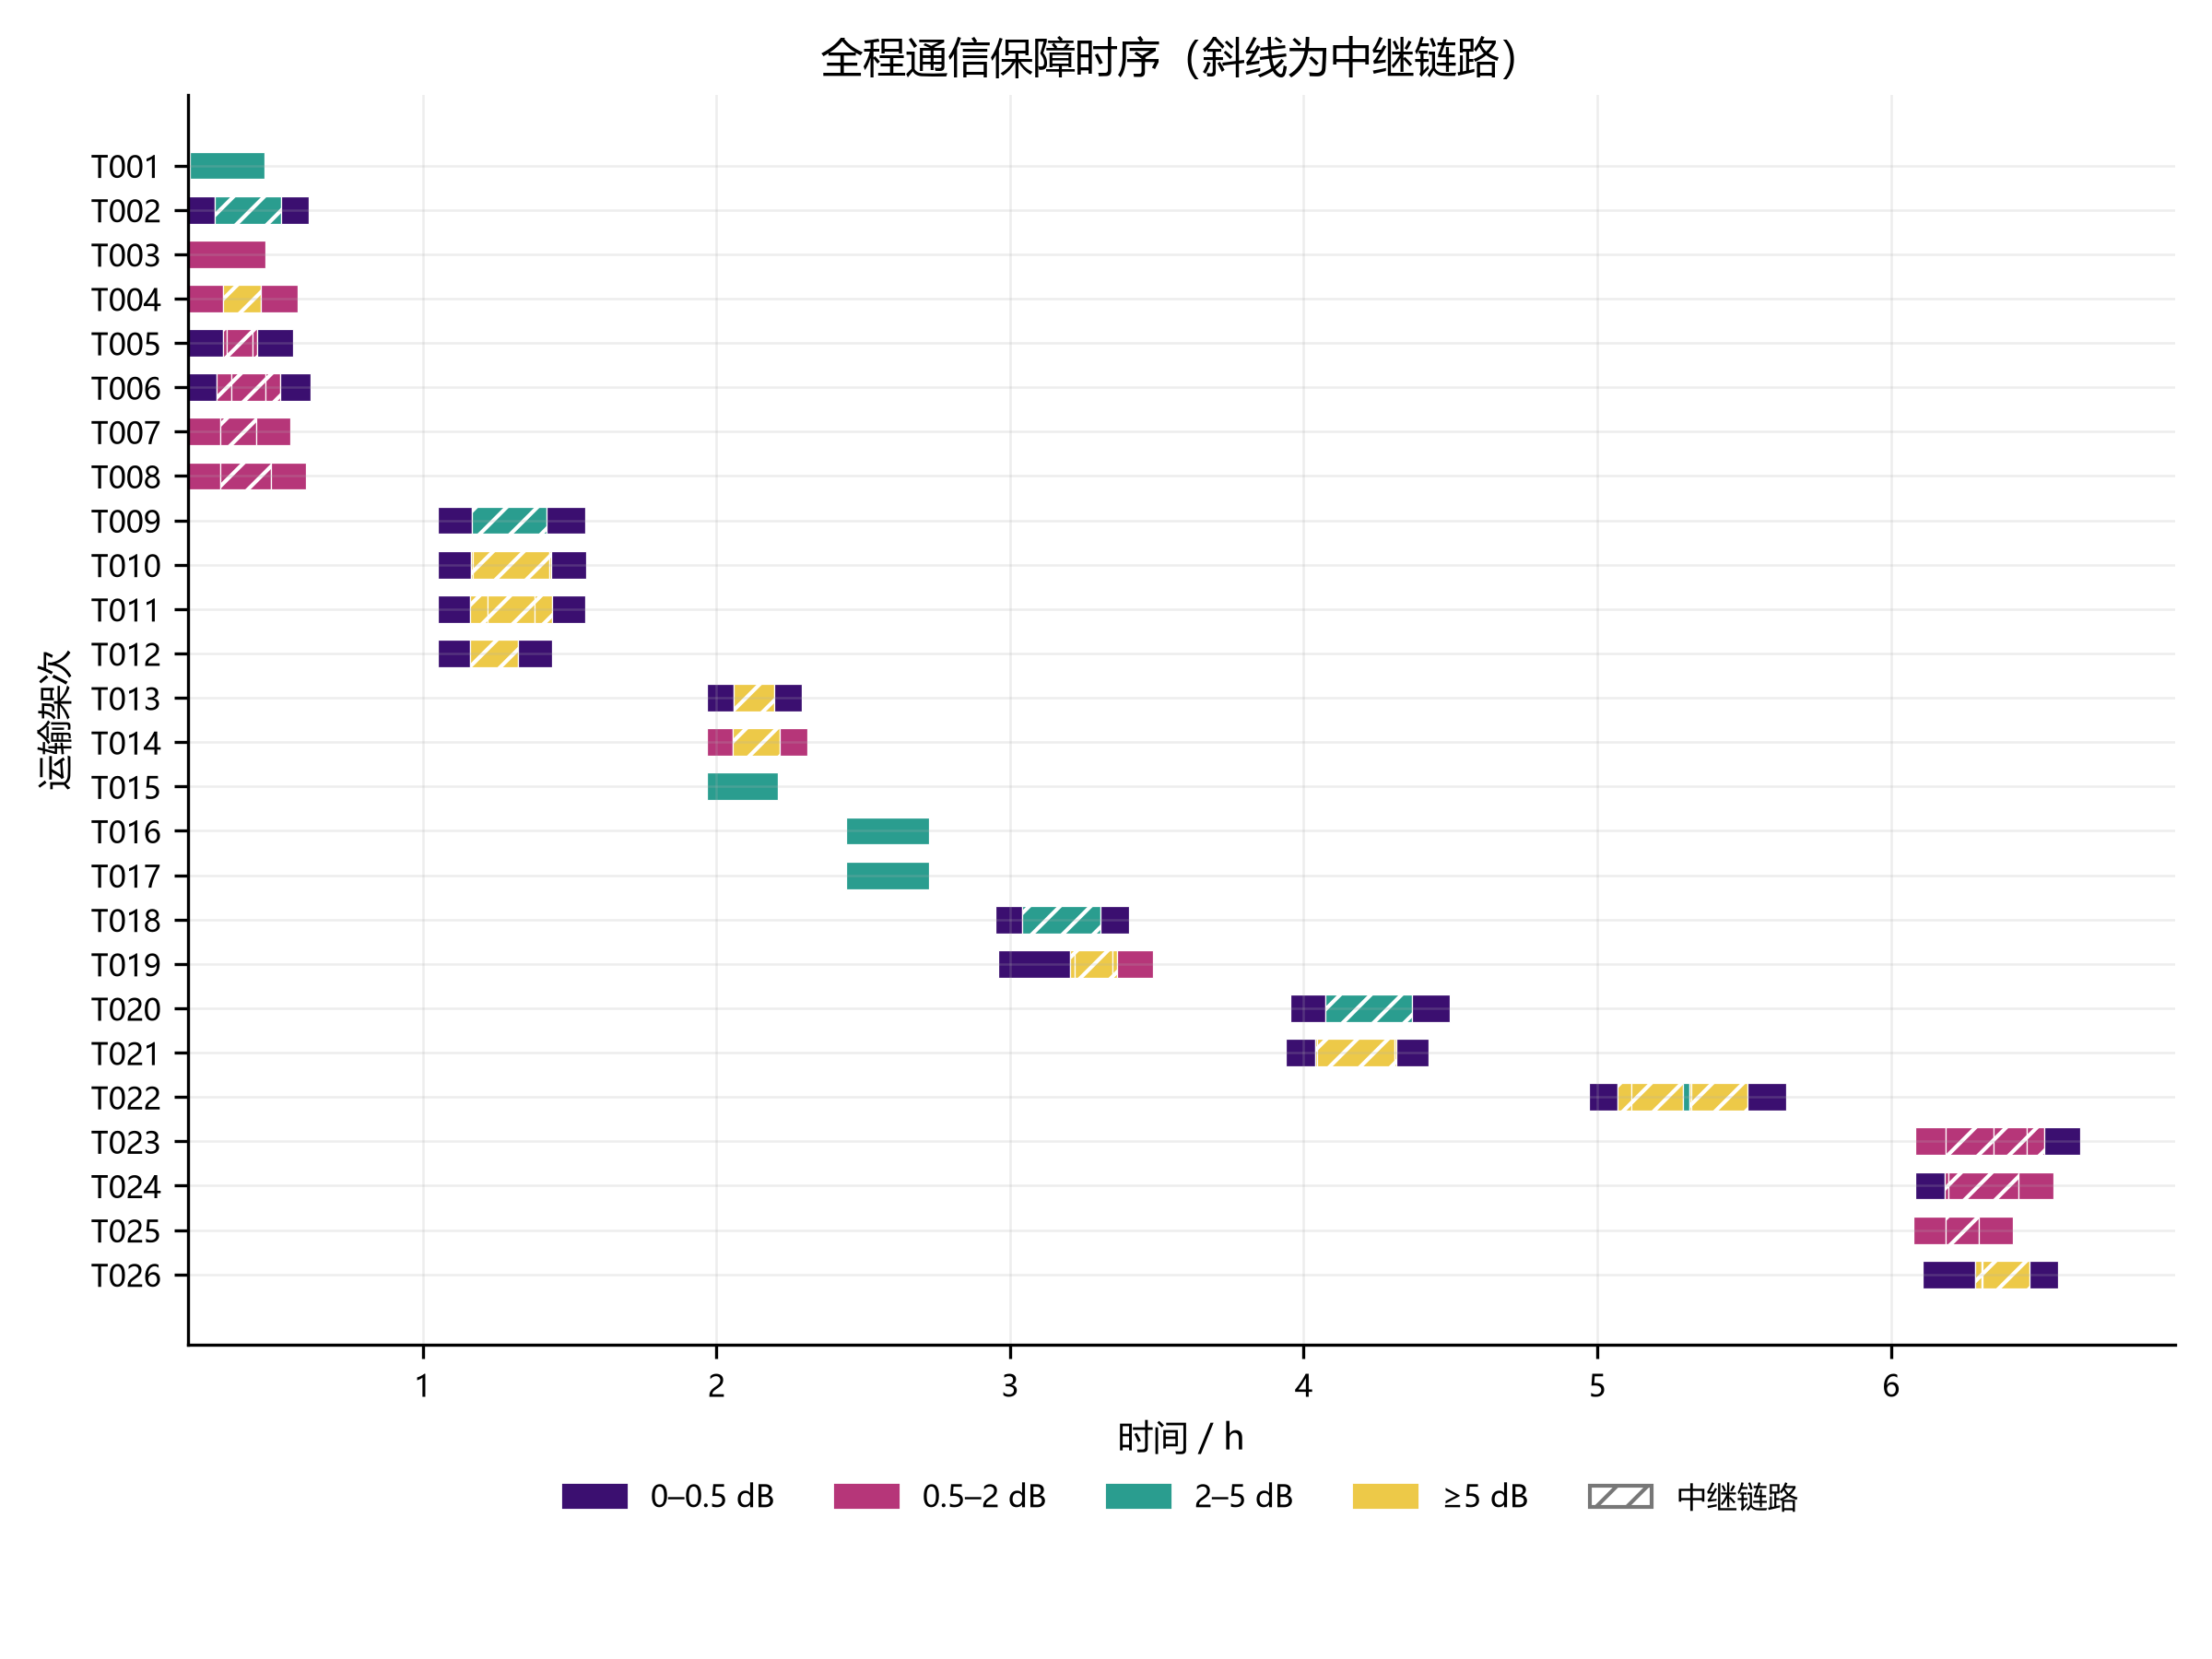
\includegraphics[width=0.98\textwidth]{figures/q3_q4/result_q3_communication_timeline.png}
\caption{22个运输架次的全程通信保障时序}
  \label{fig:q3-timeline}
\end{figure}

\paragraph{通信保障代价}
中继能耗为$9.495539\ \mathrm{kWh}$，与运输能耗$69.601587\ \mathrm{kWh}$相加得到
\begin{equation}
E^{joint}=69.601587+9.495539=79.097126\ \mathrm{kWh}.
\end{equation}
通信约束没有改变既定运输路线的飞行能耗，但波次平移使一般物资超期箱数由9箱增至32箱，$WTD$由38.787增至297.276。该结果表明，当前联合方案首先满足硬时限和连续通信，后续仍可在不改变路线的条件下压缩波次等待时间。

从增量角度看，通信保障增加了9.496~kWh能耗，占联合总能耗的12.0\%；联合完成时间相对问题二运输完成时间增加3.893~h。时间增量明显大于能量增量，说明当前方案的主要代价来自等待中继就位和波次协调，而不是中继飞行本身。优化空间因此更可能出现在波次起始时刻、候选点覆盖复用和中继资源衔接，而非单纯降低悬停功率。

\subsection{链路裕量诊断与实施边界}
\paragraph{附加损耗敏感性}
在已通过的连续证书上统一扣除附加链路裕量，可判断现有证书能否继续提供保证，结果见表\ref{tab:q3-margin}。附加裕量为0.1 dB时22个架次的原证书仍全部有效；提高到0.2 dB后仅16个架次保留原证书。这里的“未保留”表示需要重新搜索悬停点并重新认证，并不等同于已经发生通信中断。
\begin{table}[htbp]
  \centering
  \caption{附加链路裕量下的连续证书保留情况}
  \label{tab:q3-margin}
  \begin{tabular}{rrrr}
    \toprule
    附加裕量/dB & 保留证书架次 & 需重新认证架次 & 最差调整余量/dB \\
    \midrule
    0.0 & 22 & 0  &  0.140 \\
    0.1 & 22 & 0  &  0.040 \\
    0.2 & 16 & 6  & -0.060 \\
    0.5 & 8  & 14 & -0.360 \\
    1.0 & 4  & 18 & -0.860 \\
    2.0 & 3  & 19 & -1.860 \\
    \bottomrule
  \end{tabular}
\end{table}

\paragraph{工程解释与适用边界}
若实测后附加损耗超过0.1 dB，应重新搜索更高且合法的悬停点或增加靠近薄弱航段的候选点，而不能仅延长中继服务时间；后者无法改善由几何遮挡和链路预算造成的余量不足。

最小余量0.1397~dB表明当前方案在题设传播模型下可行，但通信稳健性偏紧。DEM只描述地形，未显式包含树木、建筑、降雨和小尺度多径；实际部署前应进行现场链路测量，并把测得的附加损耗重新代入连续认证。若现场要求更大的工程余量，还需要重新选点或增加中继，而不能把本题计算值直接视为飞行许可。

\section{问题四：固定联合方案下的任务分区与资源配置}
\subsection{不可拆任务块与合法分区}
问题四的输入是问题三已经确定的联合方案，不能通过重排访问顺序或移动任务时刻降低资源需求。以15个服务区为顶点，若某运输架次同时访问两个服务区，则在两顶点之间连边。同一连通分量内的服务区由共访关系直接或间接连接，必须作为不可拆的原子任务块。

冻结路线共形成11个原子任务块。图\ref{fig:q4-atoms}中灰线表示多点架次产生的共访边，相同颜色表示属于同一连通分量；没有连边的服务区各自构成单点原子块。
\begin{figure}[htbp]
  \centering
  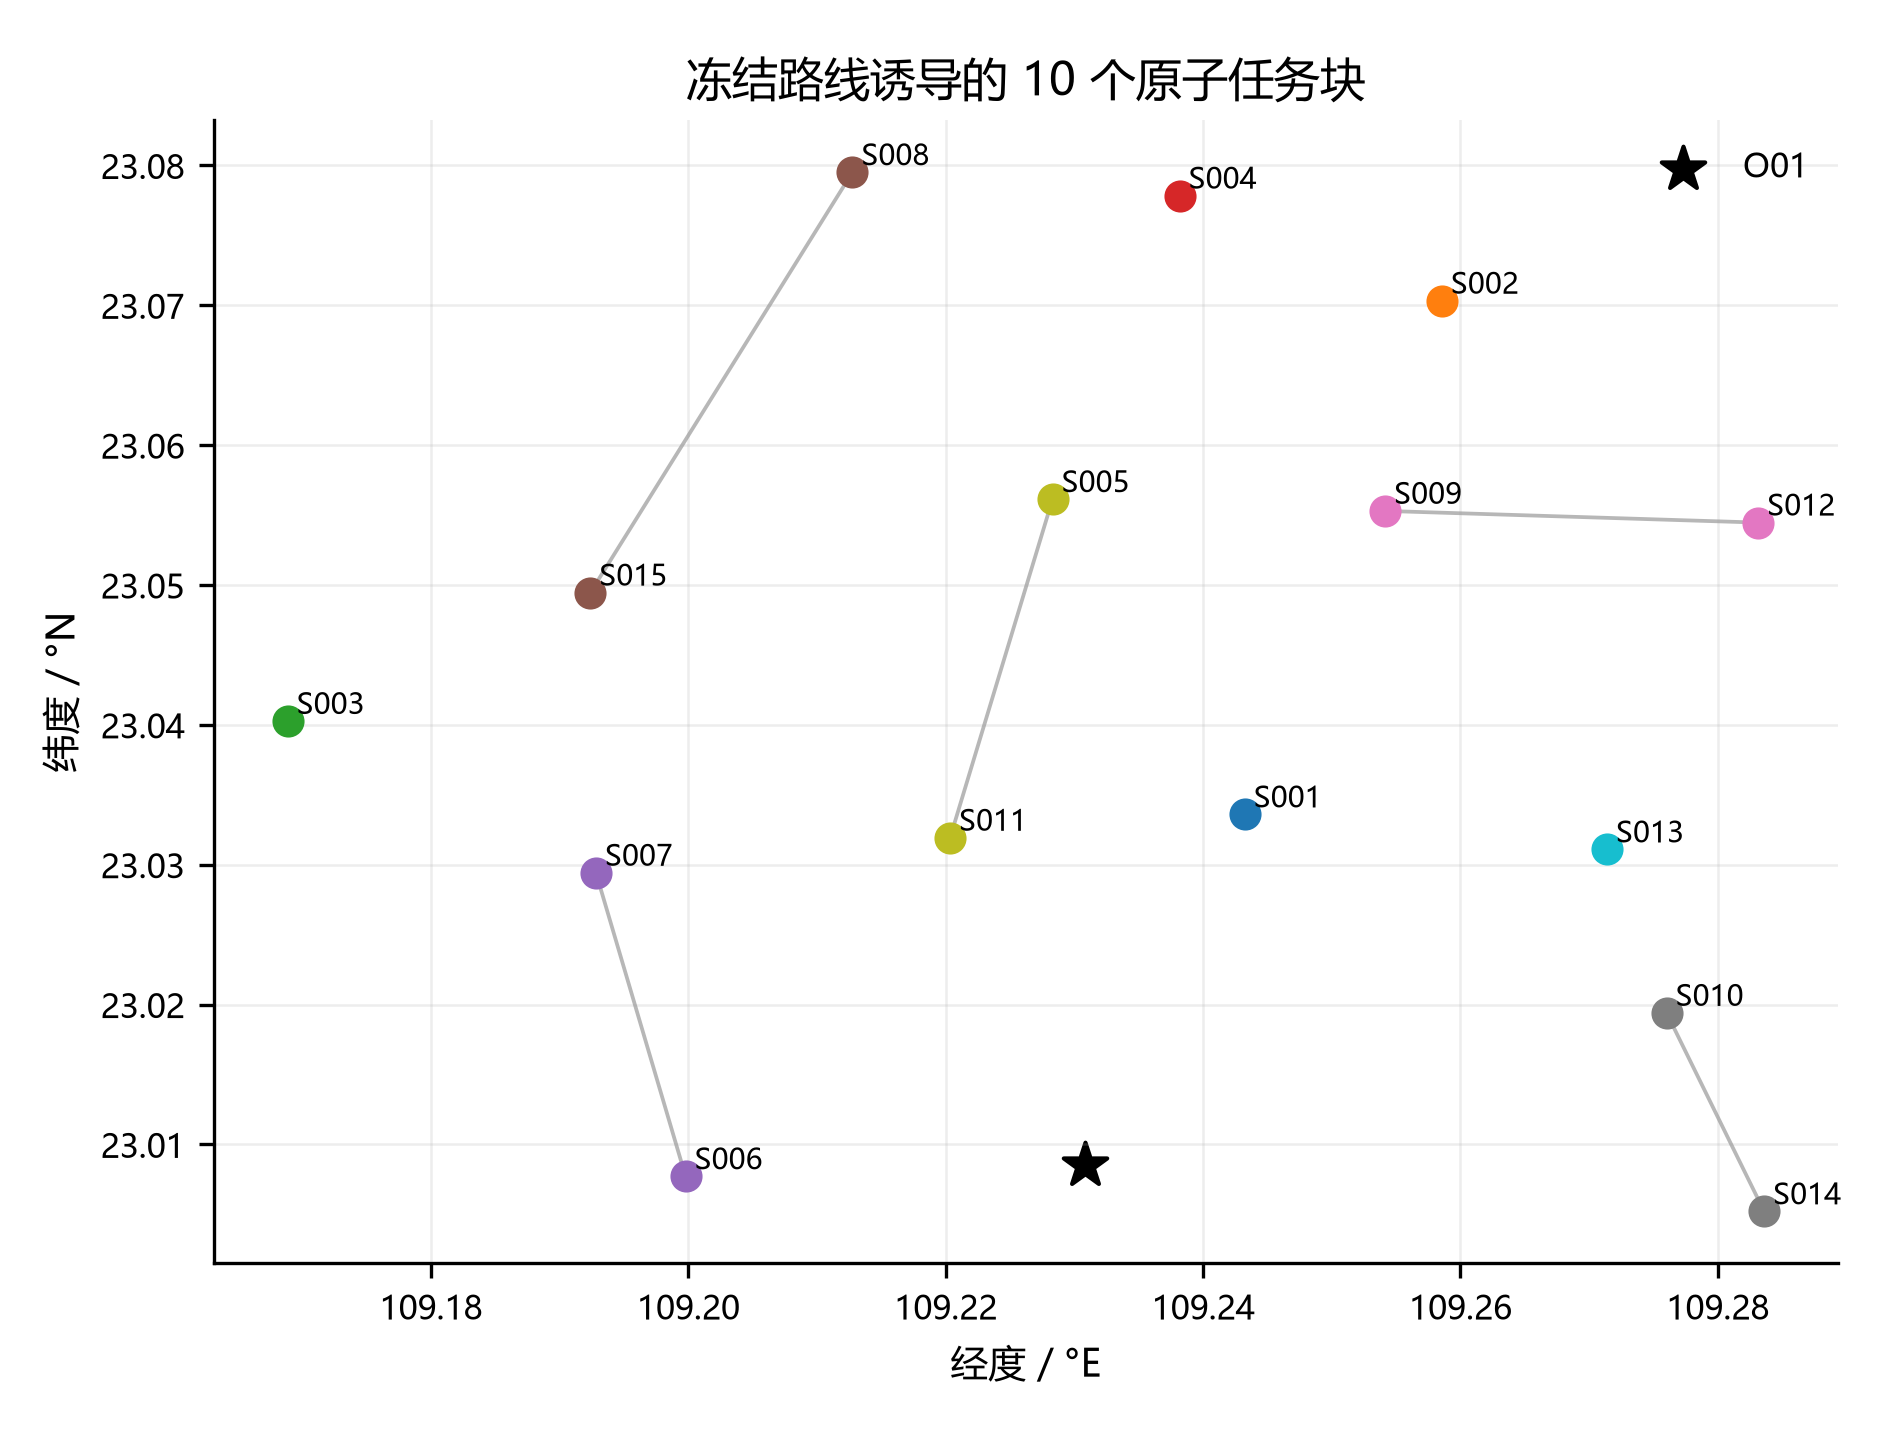
\includegraphics[width=0.78\textwidth]{figures/q3_q4/raw_q4_atomic_components.png}
  \caption{冻结运输路线诱导的11个原子任务块}
  \label{fig:q4-atoms}
\end{figure}

设原子块集合为$\mathcal A=\{A_1,\ldots,A_m\}$，将其划分为$K=2$或3个非空组。令$x_{jk}\in\{0,1\}$表示原子块$j$归属组$k$，则
\begin{equation}
\sum_{k=1}^{K}x_{jk}=1\quad(j=1,\ldots,m),\qquad
\sum_{j=1}^{m}x_{jk}\ge1\quad(k=1,\ldots,K).
\end{equation}
若$m<K$，则该固定运输方案不支持要求的非空分区。原子块由实际路线决定，不能为了获得均衡地图而拆开共访服务区。

\subsection{从实际通信分段确定中继归属}
令$\mathcal R_k$为组$k$承担的运输架次集合，$\mathcal E$为问题三最终通信分段表中出现的“运输架次—中继架次”实际指派关系。该组所需中继任务为
\begin{equation}
\mathcal H_k=\{h:\exists r\in\mathcal R_k,\ (r,h)\in\mathcal E\}.
\label{eq:actual-relay}
\end{equation}
一架中继在某波次内在位，不意味着它实际保障了波次中所有运输任务。必须从通信分段的实际指派提取$\mathcal E$，而不能把整个波次的运输架次清单直接作为保障关系。

若同一中继任务属于多个$\mathcal H_k$，各相关组独立配置资源，并保留其完整悬停点和完整原任务时段。这样既保持题设任务安排不变，又避免把并未服务本组的中继任务错误计入本组。图\ref{fig:q4-flow}给出这一资源归属链。
\begin{figure}[htbp]\centering
\begin{tikzpicture}[node distance=8mm]
\node[block,text width=5.2cm](route)at(0,0){固定运输路线\\建立服务区共访图};
\node[block,text width=5.2cm](comm)at(6,0){最终通信分段\\提取实际运输—中继关系};
\node[block,text width=5.2cm,below=of route](atom){共访连通分量\\形成不可拆原子块};
\node[block,text width=5.2cm,below=of comm](relay){确定各组关联中继\\保留完整任务时段};
\node[block,text width=11.5cm](peak)at(3,-3.4){枚举合法分区；按类型计算无人机、能源资源占用区间峰值};
\node[block,text width=11.5cm,below=of peak](out){比较配置规模、相对集中执行的冗余、库存缺口与工作量均衡};
\draw[edge](route)--(atom);\draw[edge](comm)--(relay);
\draw[edge](atom)--(atom.south|-peak.north);\draw[edge](relay)--(relay.south|-peak.north);
\draw[edge](peak)--(out);
\end{tikzpicture}
\caption{固定方案分区与资源核算流程；不代表已求得的具体服务区分组}\label{fig:q4-flow}
\end{figure}

\subsection{固定时序的最小独立资源数}
对组$k$和资源类型$a$，设必须执行的占用区间集合为$\mathcal I_{ka}$。同型资源可互换、各任务时刻固定且没有额外资源专属约束时，最小配置数等于区间峰值并发数：
\begin{equation}n_{ka}=\max_t\sum_{I\in\mathcal I_{ka}}\ind_I(t).\label{eq:peak}\end{equation}
原因是任何同时占用的区间都必须使用不同实体；反过来，按开始时刻排序、结束后回收资源的贪心分配可用峰值数量完成所有区间。

对运输机按机型分别统计任务区间，对运输电池计入任务后的完整充电；对中继机计入周转，对能源组件计入充电。所有区间采用左闭右开约定，同一时刻结束事件优先于开始事件处理。若未来增加资源专属兼容性、共享充电工位或不同初始SOC，峰值数量不再自动构成充分条件，应扩展资源模型。

\subsection{库存缺口、冗余与组间均衡}
设$I_a$为全局库存，$n_a^{central}$为同一有效联合方案集中执行所需的资源，则
\begin{equation}
D_a^{(K)}=\max\left(0,\sum_kn_{ka}-I_a\right),\qquad
R_a^{(K)}=\sum_kn_{ka}-n_a^{central}.\label{eq:shortage}
\end{equation}
前者描述资源采购或增援缺口，后者描述分区独立执行相对集中执行新增的配置。不能让每个组分别减去一份完整全局库存，也不能把“库存剩余”称为分区冗余。

以组内运输机任务占用时长和中继机含周转的占用时长之和定义工作量$W_k$，不把能源充电时间再次计作无人机机时。均衡性采用总体标准差口径：
\begin{equation}
\bar W=\frac1K\sum_kW_k,\qquad
CV_W=\frac{\sqrt{K^{-1}\sum_k(W_k-\bar W)^2}}{\bar W}.
\end{equation}
另以各组最后返航时刻之差评价完成时间均衡。两者回答不同问题：机时相近的组仍可能因等待或晚开始而较晚结束。

\subsection{分区搜索与比较原则}
按固定顺序逐一分配原子块，并以首次出现的组编号规范化消除标签对称。在每个合法分区上构造$\mathcal R_k$及$\mathcal H_k$，由式\eqref{eq:peak}计算资源向量，再比较缺口、总配置数量、$CV_W$和组间完成时刻极差。跨类型合计仅表示“件数优先”的一种建模偏好，不代表不同资源采购价格相同；同时应完整报告分类型向量，以免合计掩盖资源差异。

对$K=2$固定第一个原子块的标签后，共枚举1023个无重复分区；对$K=3$枚举57002个带标签方案，第2、3组互换后对应28501个无标签分区。全部候选均从通信分段中提取实际“运输架次---中继架次”关系，再计算固定时间轴上的资源峰值。

\subsection{两组与三组的最优分区}
表\ref{tab:q4-groups}给出两种组数下的最优分区及独立资源配置。$K=2$时S001单独组成第1组，其余14个服务区组成第2组；$K=3$时S001和S014分别组成第1、3组，其余13个服务区组成第2组。
\begin{table}[htbp]
  \centering
  \caption{两组与三组最优分区的独立资源配置}
  \label{tab:q4-groups}
  \small
  \begin{tabularx}{\textwidth}{ccYccccl}
    \toprule
    $K$ & 组 & 服务区 & A/B/C型无人机 & A/B/C型电池 & 中继机/组件 & 工作量/h & 完成时刻/s \\
    \midrule
    2 & 1 & S001 & 0/0/1 & 0/0/1 & 0/0 & 0.8858 & 11480.892 \\
    2 & 2 & 除S001外其余14点 & 4/2/1 & 4/3/2 & 2/4 & 20.2107 & 23658.349 \\
    \midrule
    3 & 1 & S001 & 0/0/1 & 0/0/1 & 0/0 & 0.8858 & 11480.892 \\
    3 & 2 & 除S001、S014外其余13点 & 4/1/1 & 4/2/2 & 2/4 & 19.6916 & 23658.349 \\
    3 & 3 & S014 & 0/1/0 & 0/1/0 & 1/1 & 1.4426 & 3024.840 \\
    \bottomrule
  \end{tabularx}
\end{table}

图\ref{fig:q4-tradeoff}按资源类型分别比较库存缺口和相对集中执行的冗余。$K=2$的各类资源总需求均不超过库存，且与集中执行的峰值需求相同；$K=3$需增配1架中继无人机，中继能源组件虽无库存缺口，但相对集中执行多配置1套。关键资源结果见表\ref{tab:q4-resource}。
\begin{figure}[htbp]
  \centering
  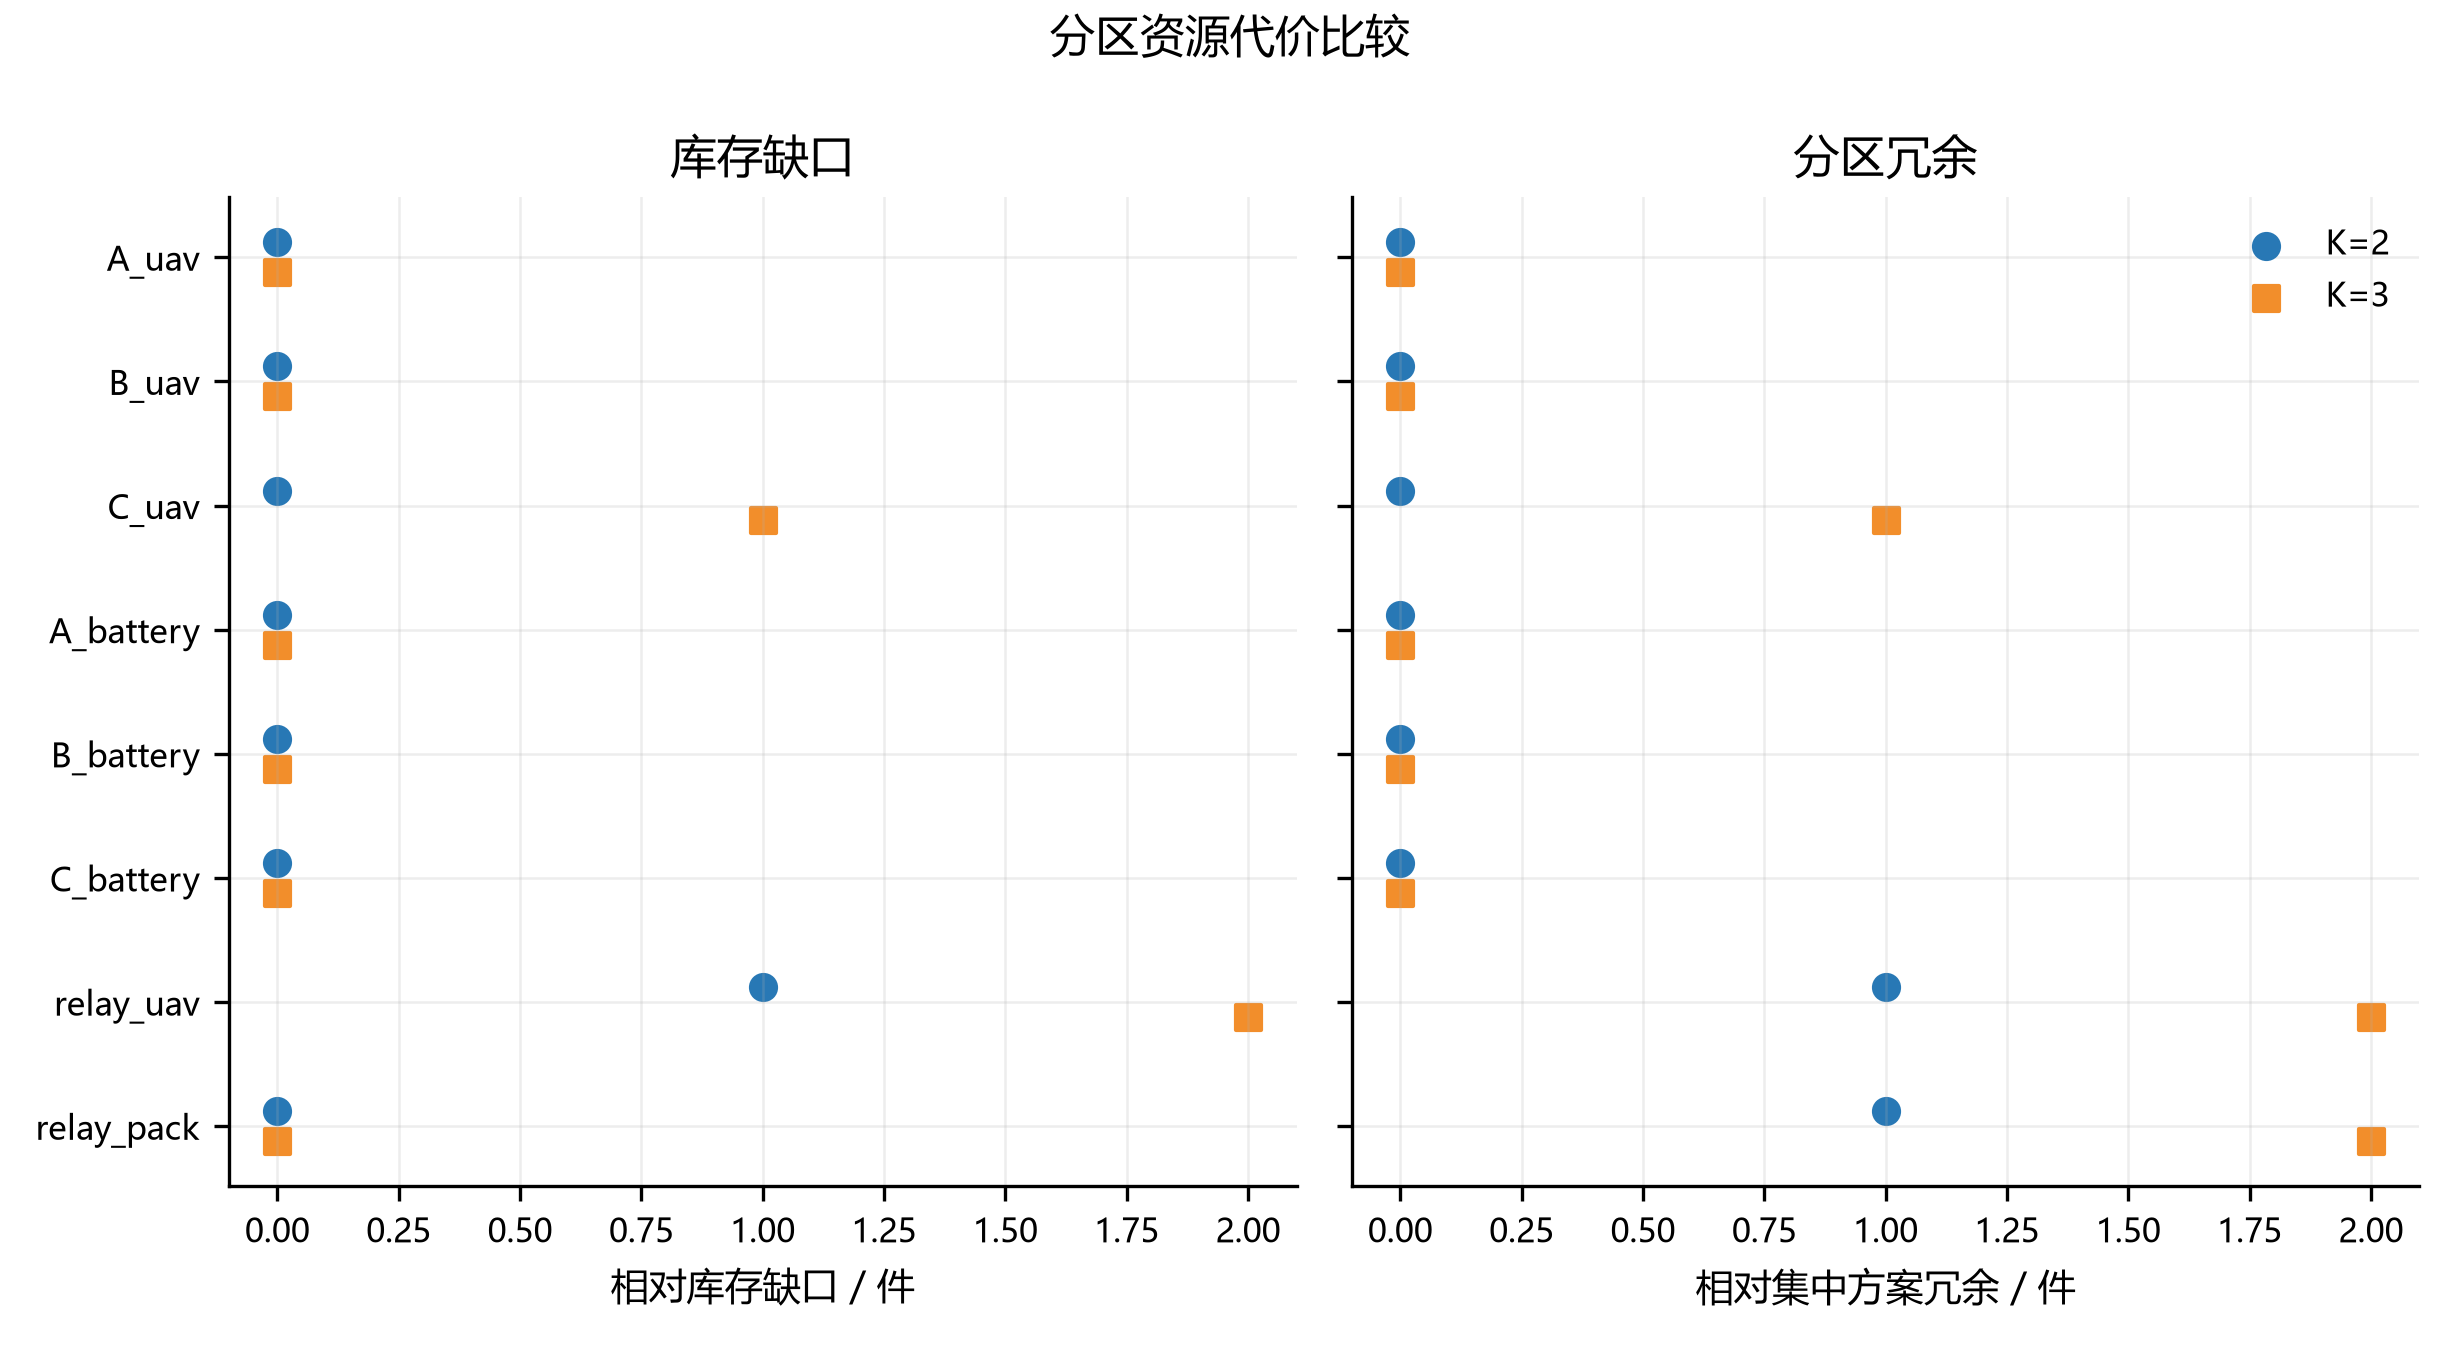
\includegraphics[width=0.98\textwidth]{figures/q3_q4/process_q4_resource_tradeoff.png}
  \caption{两种分区规模的库存缺口与相对集中方案冗余}
  \label{fig:q4-tradeoff}
\end{figure}

\begin{table}[htbp]
  \centering
  \caption{产生缺口或冗余的关键资源}
  \label{tab:q4-resource}
  \begin{tabular}{clrrrrr}
    \toprule
    $K$ & 资源 & 分组总需求 & 库存 & 缺口 & 集中需求 & 分区冗余 \\
    \midrule
    2 & 中继无人机 & 2 & 2 & 0 & 2 & 0 \\
    2 & 中继能源组件 & 4 & 6 & 0 & 4 & 0 \\
    3 & 中继无人机 & 3 & 2 & 1 & 2 & 1 \\
    3 & 中继能源组件 & 5 & 6 & 0 & 4 & 1 \\
    \bottomrule
  \end{tabular}
\end{table}

图\ref{fig:q4-map}给出最优分区的空间位置。空间邻近并不是唯一标准：不可拆性由冻结路线的共访关系决定，资源代价则由运输和通信任务在固定时间轴上的峰值并发决定。
\begin{figure}[htbp]
  \centering
  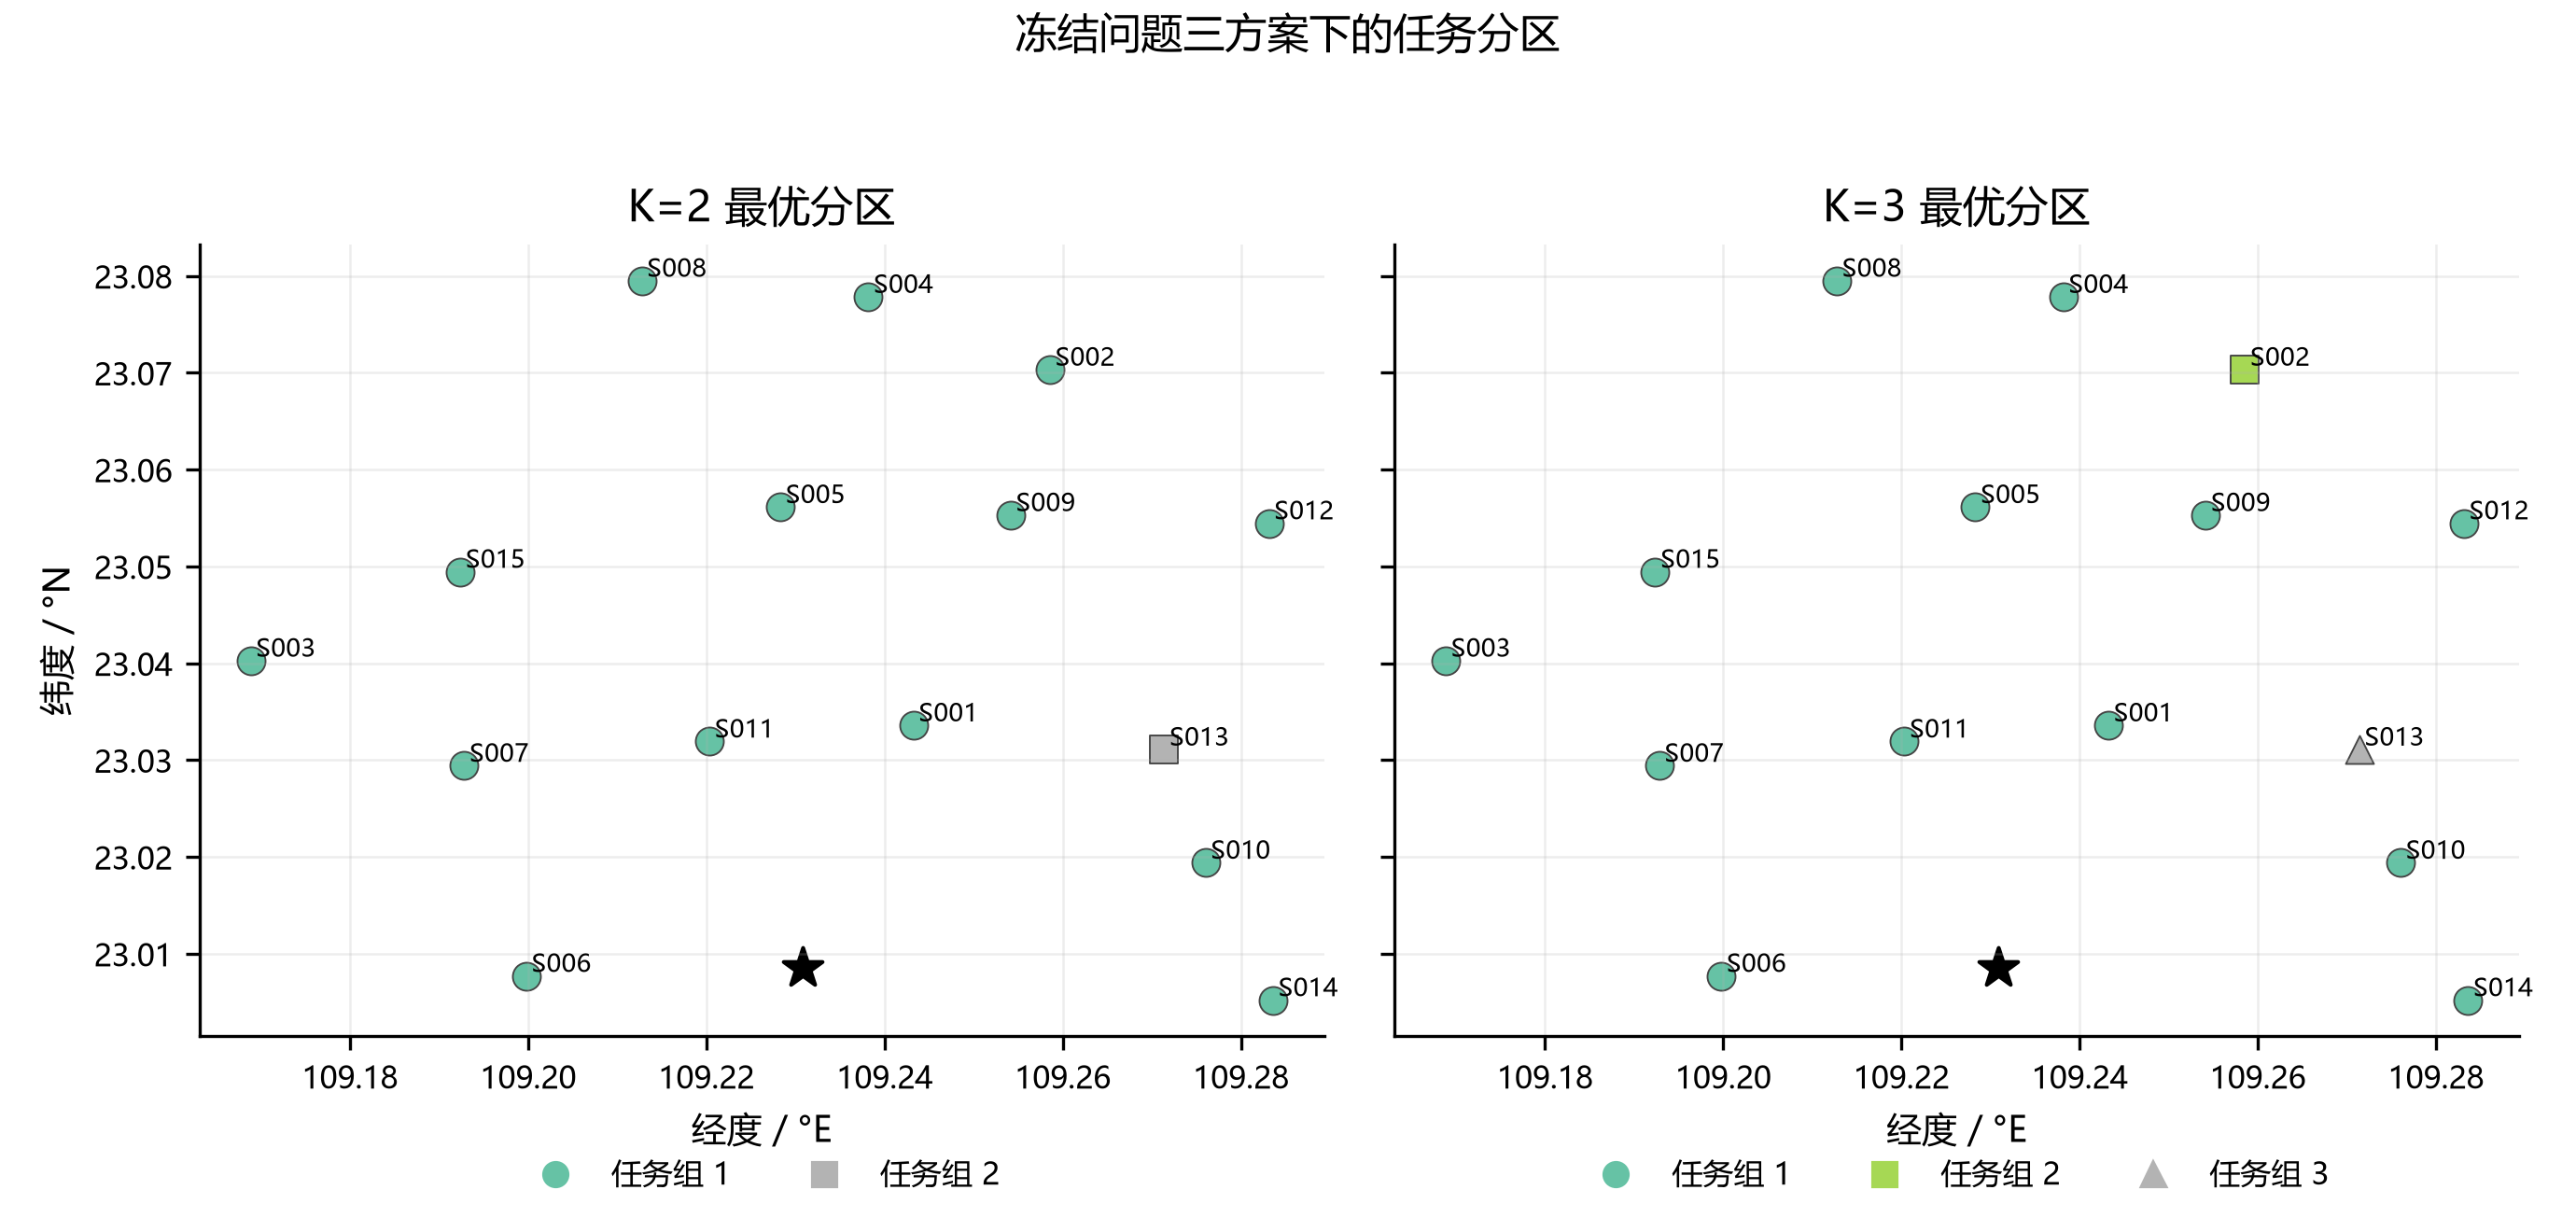
\includegraphics[width=0.98\textwidth]{figures/q3_q4/result_q4_partition_map.png}
  \caption{固定问题三方案下的$K=2$与$K=3$最优任务分区}
  \label{fig:q4-map}
\end{figure}

在“先减少库存缺口，再减少总配置和冗余”的字典序下，$K=2$优于$K=3$：前者无需增配资源，后者缺少1架中继无人机。$K=2$两组工作量分别为0.8858 h和20.2107 h，均衡性较弱，说明资源可实施性与区域负荷均衡存在明显冲突。若管理目标更强调区域自治或负荷均衡，应调整目标优先级，并接受额外的中继资源配置。

\section{算法实现与计算流程}
\subsection{公共数据结构与计算接口}
\paragraph{对象化数据组织}
为保证四问口径一致，程序不直接在各问题中重复读取工作簿，而是先构造节点、货箱、机型、实体资源、航段和通信端点六类对象。节点对象保存经纬度、地面海拔与作业高度；货箱对象保存目的地、质量、体积、类别、优先系数及适用时限；机型对象保存容量、速度、航程、能量与作业时间参数；实体资源对象保存类型、编号和下一可用时刻。

航段计算由起终点、水平距离、穿越DEM像元、最高地形、巡航海拔、爬升和下降高度组成。当前实现通过同一物理函数统一计算这些量，但没有把节点对几何结果持久缓存；不同机型和载荷会重新调用该函数，以保证时间与能耗口径一致。通信端点在此基础上增加天线高度和随时间变化的位置，使运输与通信使用相同的地形和坐标口径。

\paragraph{统一路线评价函数}
任意运输候选均交给同一个路线评价函数。输入为机型、货箱集合、访问顺序和准备开始时刻，函数按以下顺序计算：
\begin{enumerate}
  \item 汇总起飞质量与体积，检查额定容量；
  \item 根据准备和逐箱装载时间得到起飞时刻；
  \item 逐航段读取地形、计算飞行时间与当前剩余载荷能耗；
  \item 到站后按硬截止、优先系数和编号确定交接次序；
  \item 记录每箱交付完成时刻并扣除已交付质量；
  \item 计算末站返航、总能耗、返航SOC和电池充电结束时刻；
  \item 返回可行标志、全部事件和目标指标。
\end{enumerate}
问题一把路线限制为单点往返，问题二允许多点序列，问题三在相同运输事件上叠加通信检查。因此，不同问题不会因为使用不同路线函数而产生能耗或时间口径差异。

\subsection{问题一求解器实现}
\paragraph{安全载荷与候选箱组}
对每个“服务区—机型”组合先执行空载和满载边界检查，再对内部边界进行60次二分。随后将该服务区的$n_i$个货箱编码为$n_i$位掩码，预先计算各掩码的质量、体积和货箱数。一个掩码只有在至少一种机型下同时通过容量和能量检查时才进入候选表。

候选表按掩码索引，保存所有可执行机型及对应能耗和作业时长。实现中不另设显式支配删除；同一覆盖状态只保留字典序代价更小的路径，因此较差候选在动态规划更新时自然淘汰，同时保留不同覆盖集合之间可能产生的组合优势。

\paragraph{状态递推与结果恢复}
动态规划状态为已经覆盖的货箱掩码$M$。从剩余货箱的最低有效位选择锚定货箱，只枚举包含该位且与$M$不相交的候选子集$S$，以避免同一批次集合因顺序不同被重复搜索。每个状态直接保存最优字典序代价及截至该状态的完整候选路径；全集状态中的路径就是最终批次。

得到完整路径后，程序汇总全部货箱编号并执行唯一覆盖审计；同时，候选进入动态规划前已经由统一物理函数完成质量、体积和返航能量检查。若某箱未被覆盖、重复覆盖或不存在全集可行状态，则整套方案判为无效。该检查用于验证状态压缩结果与原始需求是否一致。

\subsection{问题二调度器实现}
\paragraph{两套确定性任务构造}
问题二构造并比较两套方案。第一套为硬箱专送基线：先形成硬时限任务，再对剩余普通货箱按问题一方法组批，并把能够节能的两个异区单点任务贪心合并为双区串访。第二套为同目的地混装方案：在保持基线紧急任务实体机指派的条件下，枚举同目的地软箱补入子集，再对剩余货箱重复精确组批和异区串访合并。双区路线同时评价两种访问顺序，只有完整路线函数返回容量和能量可行时才进入候选集。

两套候选均完整执行实体资源排程，并以$(N_{late}^{hard},WTD,C_{max},E_T,N_T)$字典序选择结果。当前程序没有实施通用的箱组拆分、同区合并或反复局部邻域迭代，因此所得方案是两种确定性构造中的较优者，而不是局部搜索收敛解或全局最优解。

\paragraph{实体机—电池事件排程}
对每类机型维护实体机最早可用时刻和同型电池满电时刻。排入一个任务时，枚举全部同型实体机—电池组合，以二者可用时刻的最大值作为最早准备开始时刻，再调用路线评价函数。各组合的硬迟到箱数、最大硬迟到、软时限代价、交付时刻、能耗和资源恢复时刻共同进入评分；程序选择评分最小的组合，并更新实体机返航时刻与电池充满时刻。硬迟到组合不会在生成时被直接删除，但会被零硬迟到组合严格支配；最终方案另行核验硬迟到为0。

全部任务排入后，把每个开始和结束事件写入按时间排序的事件流。扫描实体机区间和电池区间时，结束事件在相同时刻先于开始事件处理，保证半开区间约定一致。最后从逐箱交付表计算硬违约、软超期和$WTD$，从任务表计算完工时间、能耗和架次数，避免在搜索过程中维护的增量目标与最终明细不一致。

\subsection{问题三连续通信实现}
\paragraph{离线选点与固定波次输入}
运输路线被展开为准备后的爬升、水平巡航、下降、站内交接和返航区间。飞行区间位置按时间线性变化，交接区间位置固定。六个中继点由独立选点脚本在5~s黑障样本上离线搜索并筛选，随后将点位和W1--W7七个波次固化到主求解器；主程序要求输入恰为所选问题二的22个运输任务。这个绑定关系保证结果可复现，但也意味着当前实现不是每次运行时在线生成覆盖矩阵并贪心选点。

覆盖矩阵只服务于候选选择。选中点形成中继任务后，程序从每个运输时段读取实际中继编号，计算直连余量或两条中继链路余量的较小值，并生成通信分段。相邻且通信方式、实际中继和可用性依据相同的时段合并，最终得到68个可解释分段。

\paragraph{连续区间递归认证}
连续认证函数的输入为时间区间、运输轨迹段和候选通信方式。它先计算区间上的保守余量下界；下界非负则返回“整段通过”。若无法证明且区间长度大于0.1~s，则在中点二分并分别认证；任一子区间失败，父区间即失败。达到最小长度仍无法证明时按未认证处理，不用端点或中点样本替代证明。

递归返回的不仅是通过标志，还包括最小下界余量及其对应架次和区间。对最终方案再次按0.5~s步长展开全部运输轨迹，独立统计可用点与中断点。连续证书和网格检查分别写入结果表，二者均通过才把运输架次标记为通信可行。

\subsection{问题四分区枚举实现}
\paragraph{原子块与规范化分组}
先以服务区为顶点扫描全部运输路线：同一多点路线访问的服务区之间加入共访边，通过并查集或深度优先搜索得到连通分量。每个连通分量成为一个原子块，并保存其服务区集合、关联运输任务及由通信分段反推的中继任务。

枚举时按固定原子块顺序赋组，并把第一个原子块固定在第1组；其余原子块可取任一组标签，最后要求$K$个组均非空。由此实际遍历1023个两组候选，以及57002个三组带标签候选；后三者中第2、3组标签互换形成等价对，对应28501个无标签等价类。

\paragraph{资源扫描与方案排序}
对每个组收集分类型任务区间。运输机和电池按A/B/C型分别扫描，中继机与能源组件单独扫描；电池区间包含充电，中继机区间包含周转。将开始事件记为$+1$、结束事件记为$-1$，按“时刻、结束优先”的顺序累计，最大累计值即该类型最小配置。

各组资源向量汇总后，程序按“总库存缺口、总配置数、工作量变异系数、完成时刻极差、规范化分组”进行字典序排序；相对集中执行的冗余在选定方案后逐资源计算并报告，不进入当前排序键。程序保留最优方案的完整分类型向量与每组服务区，避免仅输出总件数而无法判断究竟缺少哪类资源。

\subsection{关键实现参数与输出接口}
表\ref{tab:implementation-parameters}列出影响数值判断和搜索边界的关键参数。参数要么直接来自题目附件，要么用于控制数值精度；算法没有通过调整这些参数改变题设物理条件。

\begin{table}[htbp]\centering
\caption{关键实现参数及其作用}\label{tab:implementation-parameters}
\small
\begin{tabularx}{\textwidth}{>{\raggedright\arraybackslash}p{3.0cm}YY}
\toprule
参数或约定 & 取值与来源 & 计算作用\\
\midrule
DEM基础分辨率 & 30~m，题目附件 & 地形净空与视线遮挡的空间基础\\
航段密集采样间隔 & 15~m，并补充像元边界交点 & 辅助枚举经过像元，不替代像元遍历\\
安全载荷二分次数 & 60次，数值精度设置 & 使质量区间远小于输出三位小数精度\\
资源区间约定 & 左闭右开、同刻结束优先 & 避免相邻任务在边界被误判重叠\\
连续认证最小区间 & 0.1~s，保守认证设置 & 未能证明的短区间按不可用处理\\
通信独立复核步长 & 0.5~s & 对连续证书结果进行高密度抽查\\
目标比较方式 & 硬可行优先的字典序 & 避免不同量纲指标由任意权重相加\\
\bottomrule
\end{tabularx}\end{table}

输出分为逐箱、逐运输架次、逐中继架次、逐通信分段和逐分区五个层次。逐箱记录用于核对覆盖和时限；架次记录用于回算能量和资源；通信分段用于证明连续保障并确定问题四的实际中继归属；分区记录保留分类型配置、缺口、冗余与均衡指标。分层输出使摘要和汇总表中的指标都能够由更细一级记录重新计算。

\section{模型检验、误差分析与评价}
\subsection{分层检验思路}
\paragraph{从公共物理量到全局方案}
验证应沿模型依赖链展开。先确认航段经过像元、作业高度和能耗单位，再核对单架次计算，之后检验全局资源与通信。若公共地形函数存在偏差，即使输出表之间完全一致，也不能据此证明任务满足50 m净空。

单架次检查包含四项：货箱质量与体积、随交付递减的剩余载荷、逐站交接时刻、累计能耗与返航SOC。全方案再检查每箱只出现一次、全部硬截止满足、实体及能源区间不重叠。问题三在此基础上对每段轨迹给出连续通信依据；问题四则重建实际保障关系，核对分组前后的固定任务和时刻。

\paragraph{检验指标的判定层次}
本文把检验结果分为“物理量正确、单任务可行、全局约束可行、目标值可回算”四层。第一层检查距离、高度、时间、能量和损耗的单位及边界；第二层检查每个运输或中继任务的容量、SOC和链路；第三层检查80箱覆盖、硬时限和资源并发；第四层从逐项结果重新汇总架次数、能耗、完工时间和资源峰值。只有四层同时通过，汇总结果才被写入正文。

这种层次能够区分两类错误：若单架次能耗不正确，应回到公共物理模型；若单架次均可行但资源区间重叠，则问题出在调度；若明细正确而摘要数字不同，则属于汇总或表述不一致。定位层次后再修正，可以避免用调整最终数字掩盖底层计算问题。

\paragraph{可行性、守恒关系与交叉复核}
\paragraph{四问关键检验}
表~\ref{tab:model-check}汇总四个问题的关键检验。覆盖守恒按货箱编号计数，要求80箱各出现一次；资源检验采用左闭右开区间扫描，结束事件先于同一时刻的开始事件处理；能量检验直接由逐航段能耗回算返航SOC，而不是使用汇总值反推。问题三同时使用连续区间证书与固定步长网格，两种方法回答“保守证明”和“独立抽查”两个不同问题。

\begin{table}[htbp]
\centering
\caption{四个问题的模型检验结果}\label{tab:model-check}
\small
\begin{tabularx}{\textwidth}{>{\centering\arraybackslash}p{0.8cm}>{\raggedright\arraybackslash}p{2.8cm}YY}
\toprule
问题 & 检验对象 & 判定准则 & 结果\\
\midrule
Q1 & 组批覆盖与返航能量 & 80箱各出现一次；每架次返航SOC不低于下限 & 通过；18架次，最小返航SOC为22.789\%\\
Q2 & 交付、时限与双资源占用 & 唯一覆盖；31个硬时限箱零违约；机体与电池区间无重叠 & 全部通过\\
Q3 & 连续通信、链路与中继资源 & 未解析区间为0；0.5~s网格中断点为0；中继机与组件无冲突 & 22条轨迹均通过，65532个网格点中断为0\\
Q4 & 分区完备性与资源公式 & 枚举非空带标签候选并核对无标签等价类；缺口、冗余逐类型复算 & $K=2$共1023个；$K=3$共57002个带标签候选，对应28501个无标签等价类\\
\bottomrule
\end{tabularx}
\end{table}

\paragraph{基线、等价公式与反向回算}
问题二还保留26架次硬箱专送基线作为对照。22架次混装方案不仅保持硬违约为0，而且$WTD$、完工时间、能耗和架次数同时下降，因此改进不是由放松硬约束获得。问题四的最小资源数由区间峰值和贪心复用两种等价口径核对；在固定时序与同型资源可互换的假设下，两者得到相同配置数。

能量方面，对每个运输架次同时保存逐航段能耗之和和返航SOC，二者应满足$SOC^{end}=1-E/E^{use}$；对问题三，运输能耗与中继能耗分别汇总后再相加，得到79.097126~kWh。时间方面，完工时间直接取最后返航事件，而不是充电结束事件；资源恢复时间则另外从全部充电事件取最大值。两种时间口径分别回算，可防止把“任务完成”和“系统完全恢复”混为一谈。

问题四还进行任务归属反向检查：对每个分组，把组内服务区映射回运输架次，再从实际通信分段映射到中继架次；所有原运输任务必须至少归属一个组，同一原子块不能跨组。对共享中继任务按独立执行规则在相关组中复制完整任务，再计算资源峰值。由此保证资源缺口确实来自分区独立性，而非漏记或错误切分任务。

\subsection{敏感性实验与解释边界}
\paragraph{实验设计与重算范围}
表\ref{tab:validation-plan}区分本次已经重算的敏感性实验和仍作为扩展方向的项目。返航余量实验重新计算安全载荷与问题一组批，地面延误实验在既定问题二事件链上逐级传播，链路保守余量实验则从连续区间证书的最小裕量出发判断原方案是否仍被认证。能耗系数扰动和中继任务局部裁剪会改变候选方案本身，本文不把它们写成已经完成的稳健性结论。
\begin{table}[htbp]\centering
\caption{敏感性实验与扩展检验范围}\label{tab:validation-plan}
\begin{tabularx}{\linewidth}{>{\raggedright\arraybackslash}p{2.3cm}YY}\toprule
实验对象 & 参数变化与重算范围 & 本文结论或状态\\\midrule
返航余量 & 10\%、15\%、20\%、25\%、30\%；重算安全载荷与组批 & 已完成：架次数依次为18、18、18、19、20\\
地面操作延误 & 0--1200~s，每60~s传播至问题二时序 & 已完成：硬逾期始终为0，最小硬时限余量降至1055.086~s\\
链路保守余量 & 额外收紧0、0.1、0.2、0.5、1、2~dB & 已完成：0.1~dB时22架次仍通过，0.2~dB时仅16架次通过旧证书\\
能耗不确定性 & 水平能耗系数及爬升效率分别扰动，先独立再联合比较 & 扩展项目：需重新判断能量可行性并重排方案\\
分区执行方式 & 主方案保持完整中继任务；局部时段裁剪作为另行假设 & 扩展项目：需重算分类型配置、缺口、冗余与均衡\\
\bottomrule\end{tabularx}\end{table}

返航余量从10\%提高到20\%时，最优组批仍保持18架次、59.240~kWh和32798.500~s，最小返航SOC为22.789\%，说明20\%基准在当前离散装箱结构下尚未触发重组。余量增至25\%后，安全载荷集合收缩使架次数升至19，能耗升至61.190~kWh；增至30\%时进一步升至20架次和67.358~kWh。该阶梯变化说明，安全载荷是连续变化的，但完整货箱的可行子集会在临界点发生离散跳变，因此不能仅报告某个机型的连续载荷曲线。

\paragraph{地面延误传播}
地面延误不能用“全部交付时刻统一加常数”替代，因为一次延误会沿同一实体机和共享电池的后续事件传播。本次将0--1200~s附加延误按60~s步长作用于既定调度的相关事件链；所有情景下硬逾期箱数均为0，最小硬时限余量由2255.086~s线性降至1055.086~s。因测试上界仍未越过硬时限，结论只能表述为方案对1200~s以内的该类延误保持硬约束可行，不能外推为任意延误下均可行。一般物资的软时限代价和资源完全恢复时间仍会随事件推迟而增加，实际执行时应在滚动调度中更新。

\paragraph{链路保守余量}
通信鲁棒性应区分“旧保守证据不再足以保证”与“实际链路中断”。基准连续证书的最小下界裕量为0.1397~dB；额外收紧0.1~dB后，22个运输架次仍由原证书覆盖，最差调整后裕量为0.0397~dB；收紧0.2~dB后只有16个架次仍被旧证书认证，收紧0.5、1和2~dB时分别为8、4和3个。这里的“未认证”不等于已经证明断链，而表示原点位和原区间证书不足以保证更严格条件。若要构造相应鲁棒方案，必须重新执行区间验证、选点和调度，并比较新增中继能耗与联合完工时间。

三组敏感性输出与主结果一同纳入统一复核记录。它们分别回答离散组批对安全余量的响应、固定调度对事件延误的硬时限余量，以及既定通信证书对附加链路保守量的承受范围。三者没有把尚未重算的能耗系数扰动或局部中继裁剪混入已完成结论，从而保持“改变参数后重算什么”与“当前证据能证明什么”的边界。

从决策角度看，返航余量实验给出装备安全要求提高时的运输代价阶梯，延误实验给出既定资源编排能够吸收的时间缓冲，链路实验则揭示当前通信方案的最小证书余量很窄。三类结果应分别用于组批预案、现场调度和中继点位加固，不能相互替代。

\subsection{误差来源、数值精度与影响}
\paragraph{误差分类与控制方式}
模型输出的误差不能只理解为浮点舍入。对本题影响更大的，是DEM空间分辨率、传播模型简化和启发式搜索边界。表~\ref{tab:error-analysis}按“来源—当前控制—剩余影响”给出误差审计。

\begin{table}[htbp]
\centering
\caption{主要误差来源及其控制方式}\label{tab:error-analysis}
\small
\begin{tabularx}{\textwidth}{>{\raggedright\arraybackslash}p{2.5cm}YY}
\toprule
误差来源 & 当前控制与可量化精度 & 对结论的影响与处置\\
\midrule
安全载荷求根 & 二分迭代60次，质量区间远小于输出的$10^{-3}$~kg精度 & 数值误差可忽略；临界箱组仍按未四舍五入值判定\\
DEM离散 & 沿航段遍历30~m DEM经过像元并取最高地形，统一增加50~m净空 & 对给定DEM是保守的；真实小尺度障碍和高程测量误差未被附件描述，现场需以更高精度地形复核\\
时间与事件计算 & 内部以秒和双精度计算，约束比较容差为$10^{-9}$量级；表中时间通常保留$10^{-3}$~s & 展示舍入误差不超过0.0005~s，不参与可行性判断\\
连续通信认证 & 未能直接证明的区间递归二分至0.1~s并按不可用处理；另以0.5~s网格独立抽查 & 数值检查无中断，但最小保守余量仅0.1397~dB，传播模型误差比浮点误差更重要\\
能耗参数 & 采用附件确定值，水平能耗与爬升能耗逐段累计 & 未包含风场、电池老化和温度效应；返航余量敏感性显示25\%起会触发重新组批\\
组合搜索 & Q1集合划分与Q4固定方案分区为穷举/动态规划；Q2、Q3为确定性启发式 & Q2、Q3只证明当前方案可行且优于所列基线，不证明全局最优\\
\bottomrule
\end{tabularx}
\end{table}

\paragraph{空间误差的传播路径}
DEM误差首先改变航段最高地形，继而同时影响巡航海拔、爬升时间、爬升能耗和视线遮挡。若某一高程被低估，问题一可能高估安全载荷，问题二可能低估交付时间和能耗，问题三还可能把遮挡链路误判为可用，最终传播到问题四的资源需求。因此，地形不是只影响一张地图的外部数据，而是贯穿四问的公共误差源。

本文对给定30~m DEM采用经过像元最大值加50~m的保守口径，但这种保守性只针对栅格表示本身。分辨率以下的树木、建筑和临时障碍不在附件中，无法由数值算法消除。现场部署应使用更高分辨率地形或实测航线复核，并重新运行能耗和通信模型。

\paragraph{时间误差与事件传播}
准备、装载、交接、建链和周转时间以题目给定值进入事件链。单个事件偏差不仅影响当前任务，还会通过实体机或能源资源的可用时刻影响后续任务。若多个任务连续复用同一电池，早期延误会累积传播；若换用另一块已满电电池，则传播路径可能中断。因此，误差不能简单地对所有交付时刻加同一个常数。

本文地面延误实验沿实际资源前后继关系传播，能够反映这种结构，但尚未覆盖多类事件同时随机波动。更完整的随机稳健分析可为准备、交接和建链时间设定分布，采用蒙特卡洛仿真统计硬时限失效概率；在缺少分布依据时，本文不虚构置信区间。

\paragraph{算法误差与最优性边界}
问题一在每个服务区完整枚举箱组并动态规划，问题四对固定问题三方案完整枚举合法分区，两者的算法误差主要来自输入和数值计算。问题二只比较两套确定性构造，问题三使用离线筛选后固化的点位与波次；它们证明当前方案可行且优于所列基线，不代表全局最优。相应结果必须用“可行方案、相对基线改善、当前可行上界”等措辞，而不能用未证明的“全局最短”或“绝对最优”。

由此可见，计算舍入不是主要风险。问题一在20\%返航余量下最小实际返航SOC为22.789\%，数值容差不会改变可行性；问题三最小保守链路余量只有0.1397~dB，对未建模附加损耗更敏感。因此通信结论必须限定为题设传播模型和给定DEM下成立，现场部署应预留至少0.1~dB以外的工程裕量，或重新选点并认证。

\subsection{模型评价与适用边界}
\paragraph{模型优点}
模型的主要优点有三点。第一，运输、能源、通信和分区共用同一事件时间轴，避免把机体返航等同于电池恢复；第二，完整货箱、逐站剩余载荷和实际通信分段均保留到输出层，结果能够追溯到具体对象；第三，连续区间证书、敏感性重算和基线对照共同约束结论边界，而非只报告一个目标值。载荷相关无人机路径与空中通信的既有研究也强调能量、路径和链路条件的耦合\textsuperscript{\cite{Dorling2017,Zeng2016}}。

\paragraph{模型局限}
局限同样明确。问题二只在硬箱专送基线和同目的地混装方案之间择优，问题三又在冻结运输路线后执行固化的中继点位与波次，因此22个运输架次和11个中继架次均不具备全局最优性证明；联合完成时间6.572~h应理解为当前可行上界。30~m DEM与二值遮挡附加损耗无法表达树木、建筑、降雨和小尺度多径，0.1397~dB的最小链路余量提示通信方案偏紧。问题四的结论只适用于问题三的固定任务和绝对时序；若允许各组重新排程，资源缺口与均衡性需重新计算。

\paragraph{适用场景}
因此，本模型适合标准场景下的方案生成、资源核算和预案比较，不应直接替代现场飞行许可、无线电勘测与气象评估。实际执行时宜采用滚动重调度：更新天气、道路与链路观测后，重新计算剩余任务的能量、时限和中继点位。

\subsection{模型特点与可推广方向}
\paragraph{统一事件时间轴}
传统做法容易把路线优化、机体排程、电池充电和中继保障分开计算，最后才发现时间上无法拼接。本文把准备开始、起飞、逐箱交付、返航、充电、建链和周转全部表示为事件，并通过资源前后继关系传播。这一表示使问题二的运输调度可以直接扩展到问题三，也使问题四能够在不重排时刻的条件下准确计算独立资源峰值。

\paragraph{连续认证与离散复核分工}
通信方案先用离散采样快速筛选候选，再用连续区间证书判定可行，最后以更密的0.5~s网格作独立复核。三者分别承担效率、证明和查错功能，避免把“采样未发现中断”等同于“连续时间必然可用”。这一思路也可推广到地形净空、动态禁飞区或其他连续轨迹约束。

\paragraph{从可执行性到滚动优化}
当前模型输入为确定场景，输出完整任务与资源时序。实际灾害现场可采用滚动时域方式：每完成一批任务，就用最新天气、SOC、链路观测和需求变化更新剩余任务，只冻结已经开始的区间，再重新运行组批、资源排程和连续认证。这样既保留当前模型的可解释约束，又能适应现场状态变化。

\paragraph{图表与数值的一致性检查}
\paragraph{图、表与明细数据的对应}
正文结果由同一份逐架次、逐箱和通信分段数据生成，汇总指标均可逐项回算。问题一说明容量瓶颈，问题二说明交付与资源时序，问题三说明连续保障与代价，问题四说明独立分区造成的资源变化。相同指标的比较图使用一致量纲和色标；示意图不承担数值验证功能。

附录\ref{app:outputs}列出结果表保留的关键字段。这些字段同时服务计算复核与图表解释，使“图上看到的现象”能够定位到具体架次、货箱或时间区间。

本研究在信息检索、赛题理解与任务拆解、建模讨论、辅助编程、数据质量检查、图表和论文排版等环节使用了生成式人工智能工具；工具信息、代表性输入及输出处理方式见附录\ref{app:ai-usage}。

\section{方法评价与阶段性结论}
\subsection{模型的适用性与局限}
本文框架把单点能力、调度、中继和分区组织在同一套物理与资源定义之下。其可解释性来自对象层次的区分：货箱是交付最小单位，架次是飞行任务单位，实体机与电池是分别占用的资源，通信分段是实际保障关系的记录单位。这样可以定位容量不足、能源等待或中继复制的具体来源。

模型的精确性范围也具有层次。单点集合划分在候选完整时可精确求解；固定时序区间模型可精确核算资源数；多点运输和静态中继候选的联合构造仍受启发式与候选集合限制。即使连续通信检验通过，也只证明该方案满足指定传播判据，并不证明中继点位或整体目标达到全局最优。

实际救援还受到天气、定位误差、临时禁飞、充电设备条件和动态需求影响。当前模型采用附件确定参数，30米DEM不能表征全部小尺度障碍，题设传播公式也不是完整无线环境仿真。因此，得到的方案应理解为标准场景下的计划依据，其推广需要额外的气象、通信和装备实测数据。

\subsection{主要结论}
单点任务中，B型仅在S008受到能量约束，C型在5个服务区的安全载荷低于额定值；完整货箱不可拆分又使部分批次先受到体积约束。最终单点运输需18架次。多点混装和资源事件调度将运输架次数降至22，并保证31个硬时限货箱全部按时送达。

通信约束使中继在位时间成为运输可行性的组成部分。当前方案以11个中继架次保障22个运输架次，连续区间认证和加密采样均未发现中断；相应等待使一般物资迟到指标明显增大，说明联合调度仍有压缩空间。固定该方案后，运输路线形成11个不可拆原子块。两组独立执行不产生库存缺口，三组执行则需要增加1架中继无人机；资源可实施性与组间工作量均衡之间存在明显取舍。

\begingroup
\footnotesize
\bibliographystyle{unsrt}
\bibliography{references}
\endgroup
\clearpage
\appendix
\section{逐区需求与结果表口径}\label{app:outputs}
\subsection{逐服务区需求统计}
表\ref{tab:demand-details}依据逐箱清单汇总，硬时限箱按医疗与首批要求的并集计算。正文中的总质量、体积和31箱硬时限均可由该表回算。
\begin{longtable}{lrrrr}
\caption{逐服务区需求统计}\label{tab:demand-details}\\
\toprule 服务区 & 箱数 & 质量/kg & 体积/m$^3$ & 硬时限箱数\\\midrule\endfirsthead
\toprule 服务区 & 箱数 & 质量/kg & 体积/m$^3$ & 硬时限箱数\\\midrule\endhead
S001 & 15 & 154.00 & 0.394 & 3 \\
S002 & 8 & 81.00 & 0.211 & 2 \\
S003 & 8 & 81.00 & 0.211 & 2 \\
S004 & 6 & 59.00 & 0.156 & 2 \\
S005 & 6 & 59.00 & 0.156 & 2 \\
S006 & 6 & 59.00 & 0.156 & 2 \\
S007 & 5 & 45.00 & 0.129 & 2 \\
S008 & 5 & 45.00 & 0.129 & 2 \\
S009 & 3 & 25.00 & 0.067 & 2 \\
S010 & 3 & 25.00 & 0.067 & 2 \\
S011 & 3 & 25.00 & 0.067 & 2 \\
S012 & 3 & 25.00 & 0.067 & 2 \\
S013 & 3 & 25.00 & 0.067 & 2 \\
S014 & 3 & 25.00 & 0.067 & 2 \\
S015 & 3 & 25.00 & 0.067 & 2 \\
合计 & 80 & 758.00 & 2.011 & 31 \\
\bottomrule\end{longtable}


\subsection{逐箱、逐架次和通信分段的输出}
\begin{table}[H]\centering
\caption{结果记录的对象与关键字段}\label{tab:output-fields}
\begin{tabularx}{\linewidth}{p{2.6cm}Y}\toprule
记录对象 & 关键字段与解释\\\midrule
单点批次 & 服务区、货箱集合、机型、质量、体积、能耗、完整作业时长\\
运输架次 & 架次编号、访问顺序、机型、实体机、电池、准备开始、起飞、返航、能耗与SOC\\
逐箱交付 & 货箱编号、所属架次、服务区、站内交接序号、交付完成、硬截止或期望时刻\\
能源周转 & 能源编号、任务区间、返航SOC、充电开始和结束、下次分配任务\\
中继架次 & 悬停经纬度与海拔、离地高度、实体机、能源组件、抵达、建链、服务结束和返航\\
通信分段 & 运输架次、飞行或交接阶段、区间边界、直连或中继状态、实际中继编号、可用性依据\\
分区配置 & 服务区集合、关联运输及中继任务、分类型资源数、全局缺口、相对集中执行冗余与工作量\\
\bottomrule\end{tabularx}\end{table}

表\ref{tab:output-fields}中的“开始”统一指准备开始，“交付”指单箱交接完成，“任务完成”指最后返航。电池及能源组件的充电结束只用于下一任务可用性，不加入已完成任务的完工时间。各结果表由同一计算程序导出，字段口径见表\ref{tab:output-fields}。

\section{人工智能工具使用说明}\label{app:ai-usage}

\subsection{工具信息与使用范围}
本队在解题过程中使用OpenAI Codex作为辅助工具。使用信息如下：工具名称为OpenAI Codex桌面端，开发机构为OpenAI；所用模型属于GPT-5系列Codex模型。客户端未向参赛队显示每次会话所对应的精确底层快照，因此本文不虚构子版本号。公开模型资料将GPT-5-Codex说明为针对Codex智能编程任务优化、且底层快照会随平台更新的GPT-5版本；本队实际使用日期为2026年9月24日至26日，官方资料查询地址为\url{https://developers.openai.com/api/docs/models/gpt-5-codex}。

人工智能工具参与了信息检索、赛题理解与任务拆解、建模思路讨论、LaTeX排版、辅助编程、数据质量检查、图表制作和文字初稿整理。它不直接决定最终模型与结论，所有输出均作为候选材料，由队员结合题目附件、程序实算结果和约束检查决定是否采用。

\subsection{代表性输入内容与后续处理}
表\ref{tab:ai-usage}汇总主要使用场景。表中“输入内容”是对多轮交互任务的归纳，不包含队伍编号、个人信息或其他与解题无关的内容。

\begin{table}[H]
\centering
\caption{人工智能工具的主要使用场景与处理策略}\label{tab:ai-usage}
\small
\begin{tabularx}{\textwidth}{>{\raggedright\arraybackslash}p{2.6cm}YY}
\toprule
使用环节 & 代表性输入内容 & 队员的核验与后续处理\\
\midrule
信息检索 & 检索无人机载荷相关路径、带时间窗邻域搜索、空地通信和图划分的正式文献 & 仅保留可由出版社、DOI或标准组织页面追溯的文献；核对作者、题名、年份和适用范围后再引用\\
赛题理解与任务拆解 & 梳理四问的输入、输出、约束、依赖关系及容易混淆的时间口径 & 队员回到题目和附件逐项核对，并确定四问共用地形、能量、资源事件时间轴和结果字段\\
建模思路讨论 & 比较单点组批、异构调度、连续通信认证、中继排程和固定方案分区的候选方法 & 队员讨论模型假设、评价指标与求解边界；对未穷尽的搜索明确只报告可行方案，不作全局最优声明\\
辅助编程与调试 & 生成或修改数据读取、DEM航段遍历、调度、通信验证、分区枚举和结果导出代码 & 在本地运行程序，以80箱唯一覆盖、硬时限、返航SOC、资源无冲突和连续通信等约束逐项检查；结果冲突时以题目原始数据和重新计算为准\\
数据质量检查 & 对比CSV、JSON、图表和正文中的架次数、能耗、完工时间、通信分段及资源缺口 & 通过汇总回算、跨文件交叉检查和多轮复核定位差异；未经复核的数字不写入结论\\
图表与论文写作 & 生成流程图、结果图、LaTeX段落和参考文献格式的候选稿 & 队员逐问审读并提出修改，检查图文对应、术语和数值一致性，删除无法确认的表述后形成提交稿\\
\bottomrule
\end{tabularx}
\end{table}

\subsection{队员的独立判断与责任}
队员在使用人工智能工具前后持续参与问题判断和方案取舍。具体包括：根据题意确定完整货箱不可拆、返航安全余量和硬时限优先；比较问题二基线与22架次方案后选择后者；针对问题三与其他队伍结果的差异，主动质疑当前方案的最优性，并决定在本文中保留已经完整验证的可行方案，同时明确其搜索边界而不夸大全局最优性；在问题四中确认固定问题三任务及时序后再评价独立分组的资源缺口；对生成的PDF逐页检查并要求补充模型检验、误差分析、结论、文献角标和四问流程图。

最终模型选择、参数口径、结果采用和论文提交均由参赛队负责。人工智能输出不能替代题目附件、正式文献和可复现计算；对于工具给出的建议，只有在队员能够解释其含义、确认数据来源并通过程序或逻辑复核后才予以采用。

\section{关键算法源代码}\label{app:key-code}

本附录列出生成正文结果所使用的核心Python代码片段。代码取自求解脚本\texttt{solve\_d.py}的同步快照\texttt{paper/code/solve\_d.py}，保留原始行号，便于将公式、算法描述与实际实现逐项对应。为避免机械附上与结论无关的文件读写、绘图和格式转换代码，本文只收录四问的物理计算、组合优化、事件排程、连续通信认证和分区枚举核心；完整脚本与结果文件随支撑材料一并保存。

\subsection{问题一：航段能耗、安全载荷与集合划分}

代码清单\ref{lst:q1-physics}给出载荷相关等效航程、DEM航段计算、往返能耗及最大安全载荷二分。函数\texttt{leg\_metrics}每次从DEM路径像元中取最高高程并增加50~m净空，\texttt{max\_safe\_payload}在额定载荷区间内执行60次二分，因此与正文式\eqref{eq:safe-payload}使用同一口径。

\lstinputlisting[style=pythonappendix,firstline=293,lastline=345,firstnumber=293,caption={航段能耗与最大安全载荷计算},label={lst:q1-physics}]{code/solve_d.py}

代码清单\ref{lst:q1-dp}给出单服务区可行子集枚举与集合划分动态规划。候选必须同时满足质量、体积和返航能量约束；状态中保存当前最优完整路径，最低有效位锚定用于消除同一划分的排列重复。

\lstinputlisting[style=pythonappendix,firstline=357,lastline=426,firstnumber=357,caption={问题一可行箱组枚举与动态规划},label={lst:q1-dp}]{code/solve_d.py}

\subsection{问题二：多点路线递推与双资源排程}

代码清单\ref{lst:q2-route}展示多点路线的统一事件递推。程序按访问顺序逐段计算剩余载荷下的飞行能耗，在每个服务区按硬截止、优先系数和货箱编号安排交接，并返回逐箱完成时刻、返航SOC和完整阶段记录。

\lstinputlisting[style=pythonappendix,firstline=1329,lastline=1435,firstnumber=1329,caption={多点运输路线与逐箱交付时间轴},label={lst:q2-route}]{code/solve_d.py}

代码清单\ref{lst:q2-build}对应正文的两套确定性任务构造。它先形成硬时限任务，按需枚举同目的地软箱补入，再对剩余软箱调用问题一精确组批，并贪心合并能够节能的异区单点任务。

\lstinputlisting[style=pythonappendix,firstline=1490,lastline=1600,firstnumber=1490,caption={问题二基线与混装任务构造},label={lst:q2-build}]{code/solve_d.py}

代码清单\ref{lst:q2-schedule}给出实体运输机和同型共享电池的事件排程核心。资源最早可用时刻共同决定任务开始，候选评分把硬迟到放在首位，随后比较软时限代价、交付、能耗和资源恢复时间。

\lstinputlisting[style=pythonappendix,firstline=1603,lastline=1692,firstnumber=1603,caption={运输机—电池组合生成与任务排程核心},label={lst:q2-schedule}]{code/solve_d.py}

\subsection{问题三：链路判定、连续认证与固定波次执行}

代码清单\ref{lst:q3-link}实现直连或中继链路的距离、自由空间损耗、DEM遮挡附加损耗和余量判定，是通信分段与连续认证共同调用的基础函数。

\lstinputlisting[style=pythonappendix,firstline=477,lastline=512,firstnumber=477,caption={空地链路状态与余量计算},label={lst:q3-link}]{code/solve_d.py}

代码清单\ref{lst:q3-interval}给出单个时间区间的保守证书构造。程序把移动端点在局部平面中的轨迹包络为矩形，利用距离上界和经过DEM像元集合形成最坏情形链路余量下界；若该下界非负，则整个连续区间均可判为可用，而不是只依赖端点或中点采样。

\lstinputlisting[style=pythonappendix,firstline=709,lastline=871,firstnumber=709,caption={单区间保守链路余量证书},label={lst:q3-interval}]{code/solve_d.py}

代码清单\ref{lst:q3-cert}给出多中继连续检查的主要入口。程序先组织所有可能改变可用性的时间边界，再对每个区间调用保守认证；无法直接证明的区间继续递归细分，最终汇总最小下界余量和未认证区间。

\lstinputlisting[style=pythonappendix,firstline=1757,lastline=1859,firstnumber=1757,caption={多中继连续区间认证入口},label={lst:q3-cert}]{code/solve_d.py}

代码清单\ref{lst:q3-wave}明确列出离线搜索后固化的六个悬停点和W1--W7七个波次，并展示中继实体机、能源组件和运输资源状态的初始化。这一清单同时限定了正文第三问的复现边界：输入必须是所选问题二的22架次方案。

\lstinputlisting[style=pythonappendix,firstline=1869,lastline=1975,firstnumber=1869,caption={问题三固定点位、波次与资源分配起始逻辑},label={lst:q3-wave}]{code/solve_d.py}

\subsection{问题四：峰值资源核算与完整分区枚举}

代码清单\ref{lst:q4-enum}先以半开区间事件扫描计算每类资源的峰值并发数，再从运输共访关系形成原子块。分区时固定第一个原子块的标签，遍历其余标签并排除空组，按总缺口、总配置、工作量变异系数和完成时刻极差选择方案，最后逐类型输出缺口与相对集中执行的冗余。

\lstinputlisting[style=pythonappendix,firstline=2092,lastline=2220,firstnumber=2092,caption={问题四资源峰值与两组、三组分区枚举},label={lst:q4-enum}]{code/solve_d.py}

\subsection{代码与正文结果的对应关系}

上述清单覆盖了正文主要数值结论的生成链条：问题一的18架次来自清单\ref{lst:q1-dp}；问题二的22架次及逐箱时限由清单\ref{lst:q2-route}--\ref{lst:q2-schedule}产生；问题三的11个中继架次和连续通信证据由清单\ref{lst:q3-link}--\ref{lst:q3-wave}产生，其中清单\ref{lst:q3-interval}给出连续区间证书的核心；问题四的1023个两组候选与57002个三组带标签候选由清单\ref{lst:q4-enum}遍历。代码清单用于公开计算口径，不改变正文已报告的模型边界：问题一和固定方案下的问题四为精确离散求解，问题二只比较两套确定性构造，问题三采用离线搜索后固化的点位与波次。

\subsection{运行环境与执行顺序}

代码快照的SHA--256为\texttt{\seqsplit{57131c50ef5e68faf86ac7a4e9ee8e91fa3061fcfd6a07aa8319ef175011aea0}}。该摘要用于确认附录所示行号与实际执行文件属于同一版本；若代码发生修改，应重新生成结果并同步更新论文中的数值与图表。核心依赖及其用途见表\ref{tab:code-environment}。

\begin{table}[H]
\centering
\caption{核心运行依赖与用途}\label{tab:code-environment}
\begin{tabularx}{\textwidth}{p{3.0cm}p{3.0cm}Y}
\toprule
软件或库 & 固定版本 & 主要用途\\
\midrule
Python & 3.x & 主程序运行、数据结构与文件管理\\
NumPy & 2.4.6 & 数组计算、统计量与轨迹采样\\
Pandas & 2.3.3 & 工作簿读取、逐箱和逐任务表处理\\
Pillow & 12.2.0 & DEM栅格读取与像元数据转换\\
OpenPyXL & 3.1.5 & Excel附件解析支持\\
Matplotlib/\newline Seaborn & 3.11.1/0.13.2 & 结果图与敏感性图绘制\\
\bottomrule
\end{tabularx}
\end{table}

在项目根目录执行\texttt{python solve\_d.py --mode full}即可依次计算四问；程序也支持\texttt{q2}和\texttt{q34}模式，用于在运输方案更新后分别重算后续环节。执行完成后，先检查程序返回状态，再核对80箱唯一覆盖、31个硬时限箱零违约、各实体资源区间无冲突、连续通信未认证区间为0以及分区资源缺口。这些检查全部通过后，方可用输出文件更新正文汇总表。若只修改论文文字而不修改输入、参数和求解脚本，则不应改变任何结果数字；若更换DEM、时限、能源参数或固定波次，则必须从受影响的最早问题开始顺序重算，避免混用不同版本的路线、通信分段和分区资源结果。

\end{document}
